\chapter{Analise Bibliográfica sobre Inteligência Artificial e discriminação racial, por Gustavo R. dos Santos\label{chap:bibliometria:gutorsantos}}

\section{Planejamento do estudo}

Na última década, é notável o incrível avanço tecnológico que o mundo vem desenvolvendo nas mais diversas áreas do conhecimento. Entretanto, é irrefutável a importância da Ciência da Computação e suas áreas correlatas em grande parte desse avanço. Atualmente, quase todos os espaços possuem algum tipo de sistema informatizado, desde um pequeno comércio com um \textit{software} de controle de estoque até uma instituição financeira com um sistema complexo envolvendo dezenas de \textit{artefatos} diferentes. 

Nesse sentido, esse fenômeno se dá em razão de um maior acesso da população à artefatos tecnológicos, principalmente, à \textit{smartphones} mas também à computadores pessoais. Sendo que o contrário também é válido, haja vista a pandemia do covid-19 a qual obrigou diversos ambientes a implementarem algum tipo de sistema informatizado ocasionando numa alta na procura por computadores pessoais. 

É visível que uma das áreas que mais se destaca dentro da computação, atualmente, é a da \textbf{Inteligência Artificial (IA)}, sendo ou não parte de uma comunidade técnica da computação, é bem provável que, de uns anos para cá, boa parte dos usuários já tenham ouvido falar sobre. A IA se faz presente na rotina de todos os usuários mesmo que não seja percebida por eles. Estes usuários formam uma densa rede de conexões a qual gera um volume de dados descomunal, denominado \textbf{Big Data}. Dessa forma, a IA escolhe, por exemplo, qual será o melhor anúncio a ser exibido para um usuário com base em um pequeno conjunto de dados extraídos desse massivo conjunto que configura o Big Data.

Atualmente, o poder no que se refere a Inteligência Artificial concentra-se na mão de poucas empresas, as chamadas \textbf{Big Techs}. Os \textit{frameworks} mais conhecidos, como \textbf{TensorFlow}, \textbf{PyTorch}, \textbf{CNTK}, são, respectivamente, mantidos pelas empresas, Google, Facebook, Microsoft. Aliado à isso, ao longo de várias décadas, pricipalmente quando havia uma preocupação com dados, essas empresas acumularam em massa os dados dos usuários os quais utilizavam seus serviços. Em razão disso, o Orgão Antitruste da União Européia alertou que essa concentração dos dados enquadra-se como uma possível violação das regras de competitividade da EU.

Tendo isso em vista, a quantidade de informação contida no Big Data favorece a exploração desses dados com o intuito de tentar modelar algoritmos, com base em IA, que forneçam algum tipo de previsão e, ou, análise dos dados resultando numa tomada de decisão muitas vezes sem a necessidade de intervenção humana. Com isso, a IA contribui positivamente para diversos campos do conhecimento, como por exemplo, na área médica, onde é possível gerar diagnósticos rápidos e precisos com base nesses algoritmos.


Consequentemente, a introdução de um novo artefato tecnológico na sociedade ocasiona diversos impactos em diferentes esferas coletivas --- social, comportamental, econômica, cultural e medicinal, principalmente. Portanto, deveriam ser realizados estudos e debates --- como proposto por \citet{simon_jones_doing_2016}  --- acerca de quais são os efeitos ao se disponibilizar publicamente uma nova tecnologia. Sendo assim, observa-se que, na atual conjuntura, tal fato não ocorre dentro da área de IA e, também, de outras tecnologias. Há um descaso das Big Techs em promover esses estudos pois há 

Há uma idealização romântica sobre o que a Inteligência Artificial poderá vir a ser, propagam-se cenários onde carros serão autônomos, jogos eletrônicos ganharão mais realismo, detecção de doenças quadros em estágio inicial. Todos esses cenários são válidos porém apenas enfatizá-los corrobora para a construção de um imaginário coletivo irreal no qual não existem problemáticas. Portanto, não há a reflexão e conhecimento acerca dos problemas advindos desse novo artefato. Na verdade há um único debate acerca de um possível cenário não desejado, a \textit{revolução das máquinas}. Isso ocorre do produto de dois fatores, toca-se no imaginário do indivíduo e traz-se à tona referências de cultura pop da ficção científica  e da carência de informações que descrevam corretamente o que é uma Inteligência Artificial. Por mais que isso fosse real, a \textit{era das máquinas} ainda demoraria muito para ocorrer, temos problemas mais urgentes para resolver no agora.

Diante das reflexões expostas acima, o presente estudo tem como objetivo estimular a reflexão de como os algoritmos de Inteligência Artificial têm contribuído para diversos tipos de discriminações --- racial, de gênero, religiosa, por orientação sexual --- mais especificamente na \textbf{discriminação racial}. Para essa finalidade, algumas perguntas foram formuladas para guiar o estudo.

\begin{quote}

Qual a base de conhecimentos científicos produzida em torno do tema inteligencia artificial e discriminação racial?

Como a inteligencia artificial tem sido usada para corroborar com a discriminação racial? 

Quais são os principais países preocupados com esta problemática?  São eles as potências dessa nova tecnologia?

Quais os impactos da implementação dessas tecnologias para a população negra?

\end{quote}


\subsection{O que já existe de pesquisa bibliométrica sobre esse tema?}

Será explicitado mais aprofundamente ao decorrer deste artigo mas esse tema é extremamente recente e não foram encontrados estudos bibliométricos acerca do mesmo. 

\subsection{Ferramentas de apoio}

Para um enriquecimento da pesquisa, foi utilizado o pacote da linguagem R, \textbf{Bibliometrix}, o qual fornece o \textbf{Biblioshiny}, uma interface web para o Bibliometrix a qual facilita a análise e geração de gráficos dos dados inseridos. Dessa forma para um bom proveito da ferramento, foi seguido o \textit{workflow} propostos pelos autores do pacote, conforme indica a figura ~\ref{fig:bibliometrix:workflow}.

\subsection{Limitações} 
O estudo foi realizado ao longo de pouco mais de uma semana, tendo como base os conteúdos das aulas expostos dentro do ambiente de ensino. 

Os dados foram extraídos somente da base de dados Web of Science, além disso o conjunto de dados foi bem menor do que o esperado.

\section{Coleta de dados}

A coleta de dados feita usando o base de publicações científicas do Web of Science (WoS) no dia 08 de fevereiro de 2022, acessado por meio do Portal de Periódicos da CAPES.

A busca foi realizada na Coleção Principal da Web Of Science que reúne vários registros de diferentes áreas do conhecimento,

Foi usada a \textit{query} de busca ilustrada nas linhas 1 a 9 da listagem \ref{IAeDiscriminacaoQuery}.

\lstinputlisting[
    numbers=left,
    basicstyle=\normalsize\ttfamily,
    caption={Query de busca sobre Inteligência Artificial e Discriminação Racial},
    label=IAeDiscriminacaoQuery
]{experiments/gutorsantos/AnaliseBibliometrica/IAeDiscriminacao/Query/query.txt}

\subsection{Explicação para os termos de busca usados}
A busca é constituída de duas cláusulas disjuntivas unidas por uma conjunção utilizada na busca por tópico (O termo de busca pode aparecer no Título, no Abstract, na Author Keywords, ou nas Keywords Plus da referência).

Na primeira cláusula (linhas 1 a 5), temos três termos compostos de conjunções, usamos aqui as conjunções para garantir que sempre uma palavra apareça juntamente da outra --- artificial-inteligence, machine-learning, computer-vision --- não precisamos que necessariamente esses termos apareçam simultâneamente, portanto, usamos a disjunção. Inicialmente, na cláusula havia somente \textit{artificial inteligence} porém esse termo é muito genérico, dessa forma, para aumentar o número de resultados da busca utilizamos esses outros dois termos que técnicamente não são sinônimos de inteligência artificial porém no campo semântico podem exercer essa função.

De forma análoga, queremos que qualquer um desses termos citados acima aparece juntamente da segunda cláusula, por isso é explicado o uso da conjunção. (linha 6)

Na segunda cláusula (linhas 7 a 14), inserimos os termos relacionados à discriminação racial, seguindo o mesmo raciocínio dos termos da primeira cláusula, utilizamos disjunção para a ocorrência de pelo menos um dos termos. Vê-se a presença de vários termos relacionados ao radical race (raça), isso é feito para dar um direcionamento mais acertivo além disso temos três termos compostos, um deles possui uma disjunção pois apesar de terem significados diferentes podem ser usados como sinônimos, os outros dois finais (linhas 12 e 13) são compostos para evitar a ocorrência do homônimo de race que remete à corrida.

\section{Análise dos dados}

\subsection{Exportação dos registros de registros}
Foi utilizada a opção \textit{export full record} no WoS, para que as citações também fosse usadas em análises da citações (estrutura intelectual do conhecimento). 

O conjunto de dados foi intitulado de IADR, acrônimo para Inteligência Artificial e Discriminação Racial.

Os 259 registros obtidos encontram-se no GitHub do projeto, em \url{https://github.com/jhcf/Comput-Experim-20212}, no diretório { experiments / gutorsantos / AnaliseBibliometrica / IAeDiscriminacao / IADR.txt}. 

\subsection{Análise descritiva do \textit{dataset} IADR@gutorsantos}

Antes de partimos para análise, apresentaremos algumas métricas essenciais para melhor entendimento do conjunto de dados. As métricas a seguir mostram de forma direta informações básicas acerca dos dados utilizados.


\newcommand\startYearIADR{1994}
\newcommand\finalYearIADR{2022}
\newcommand\totalReferencesIADR{12.496}
\newcommand\totalKWPlusIADR{625}
\newcommand\totalKWAuthorIADR{791}
\newcommand\totalAuthors{1.210}
\newcommand\totalDocuments{259}
\newcommand\totalSource{217}

\begin{description}
    \item [\textit{Timespan}] Os artigos que atenderam aos critérios de busca e filtragem foram publicados distribuídos num intervalo de tempo de \startYearIADR{} até \finalYearIADR{}.
    \item [\textit{Sources (Journals, Books, etc)}] No dataset IADR@gutorsantos, Existem \totalSource{} fontes de informação as quais os documentos encontram-se publicados. Ou seja, em média, cada \textit{scientific journal} publicou $\startYearIADR{}/\totalSource{}=1,19$ artigos. \footnote{Note que a média, enquanto medida de tendência central, pode não ser a que melhor reflete a tendência a quantidade de artigos publicados por revista.}
    \item [\textit{Average years from publication}] A média do tempo de publicação dos artigos é de 2,6 anos.
    \item [\textit{Average citations per documents}] Cada artigo foi citado, em média 9,301 vezes\footnote{Note que a média, enquanto medida de tendência central, pode não ser a que melhor reflete a tendência de  citações a artigos.}.
    \item [\textit{Average citations per year per doc}] Após publicado, cada um dos \totalDocuments{} artigos foi citado 2,167 vezes por ano, em média.
    \item [\textit{References}] O dataset contém 12.496 referências citadas.
    \item [\textit{Keywords Plus (ID)}] 625 distintas palavras-chave do tipo Keywords Plus (ID)\footnote{\textit{KeyWords Plus} são ``termos de índice gerados automaticamente a partir dos títulos de artigos citados. Os termos do KeyWords Plus devem aparecer mais de uma vez na bibliografia e são ordenados de frases com várias palavras a termos únicos. O KeyWords Plus aumenta o número de resultados tradicional de palavras-chave ou títulos.'' Fonte: \url{https://images.webofknowledge.com/WOKRS410B4/help/pt_BR/WOS/hp_full_record.html}}
    \item [\textit{Author's Keywords (DE)}] 791 palavras-chave distintas indicadas pelos autores foram encontradas no \textit{dataset}.
    \item [\textit{Authors}] 1210 distintos nomes de autores foram encontrados no dataset\footnote{Um mesmo autor pode ter uma ou mais diferentes grafias no dataset, e serão reconhecidos dois ou mais autores diferentes, embora de fato sejam apenas um. Isso significa que a quantidade de \textbf{nomes de autores} equivale à quantidade de \textbf{autores}. Adicionalmente, é possível que distintos autores sejam reconhecidos com o mesmo nome, isso é, que sejam homônimos. Ou seja, o dataset em geral conterá erros de contagem na quantidade de autores reais.}.
    \item [\textit{Author Appearances}] Os 1.210 nomes distintos de autores foram encontrados 1.284 vezes, como autores de artigos.
    \item [\textit{Authors of single-authored documents}] Dentre estes mesmos 1.210 autores distintos encontrados, 35 deles editaram artigos individualmente, isso é, sem co-autores.
    \item [\textit{Authors of multi-authored documents}] Dentre estes mesmos 1.210 autores distintos encontrados, 1.1175 deles editaram artigos com um ou mais co-autores"
    \item [\textit{Single-authored documents}] Dentre os \totalDocuments{} documentos presentes no dataset, 35 foram escritos por um único autor, e os 224 restantes foram elaborados em co-autoria.
    \item [\textit{Documents per Author}] Dentre os 19.410 distintos (nomes de) autores, cada um publicou em média 0,214 artigos.
    \item [\textit{Authors per Document}] Cada um dos \totalDocuments{} documentos presentes no dataset foi autorado com 4,67 autores em média ($1.210 / 259 = 4,67$).
    \item [\textit{Co-Authors per Documents}] As 1.284 aparições de autores (``Author Appearances''), se distribuem, em média 4,96 vezes para os \totalDocuments{} documentos do dataset.
    \item [\textit{Collaboration Index}] Os 1.210 autores que editaram artigos com um ou mais co-autores, colaboraram em media 5,25 vezes para editar os 224 artigos elaborados em co-autoria, gerando, assim, um índice de colaboração 5,25. 
\end{description}

\subsection{Evolução da Produção Científica}

\begin{figure}[!h]
    \centering
    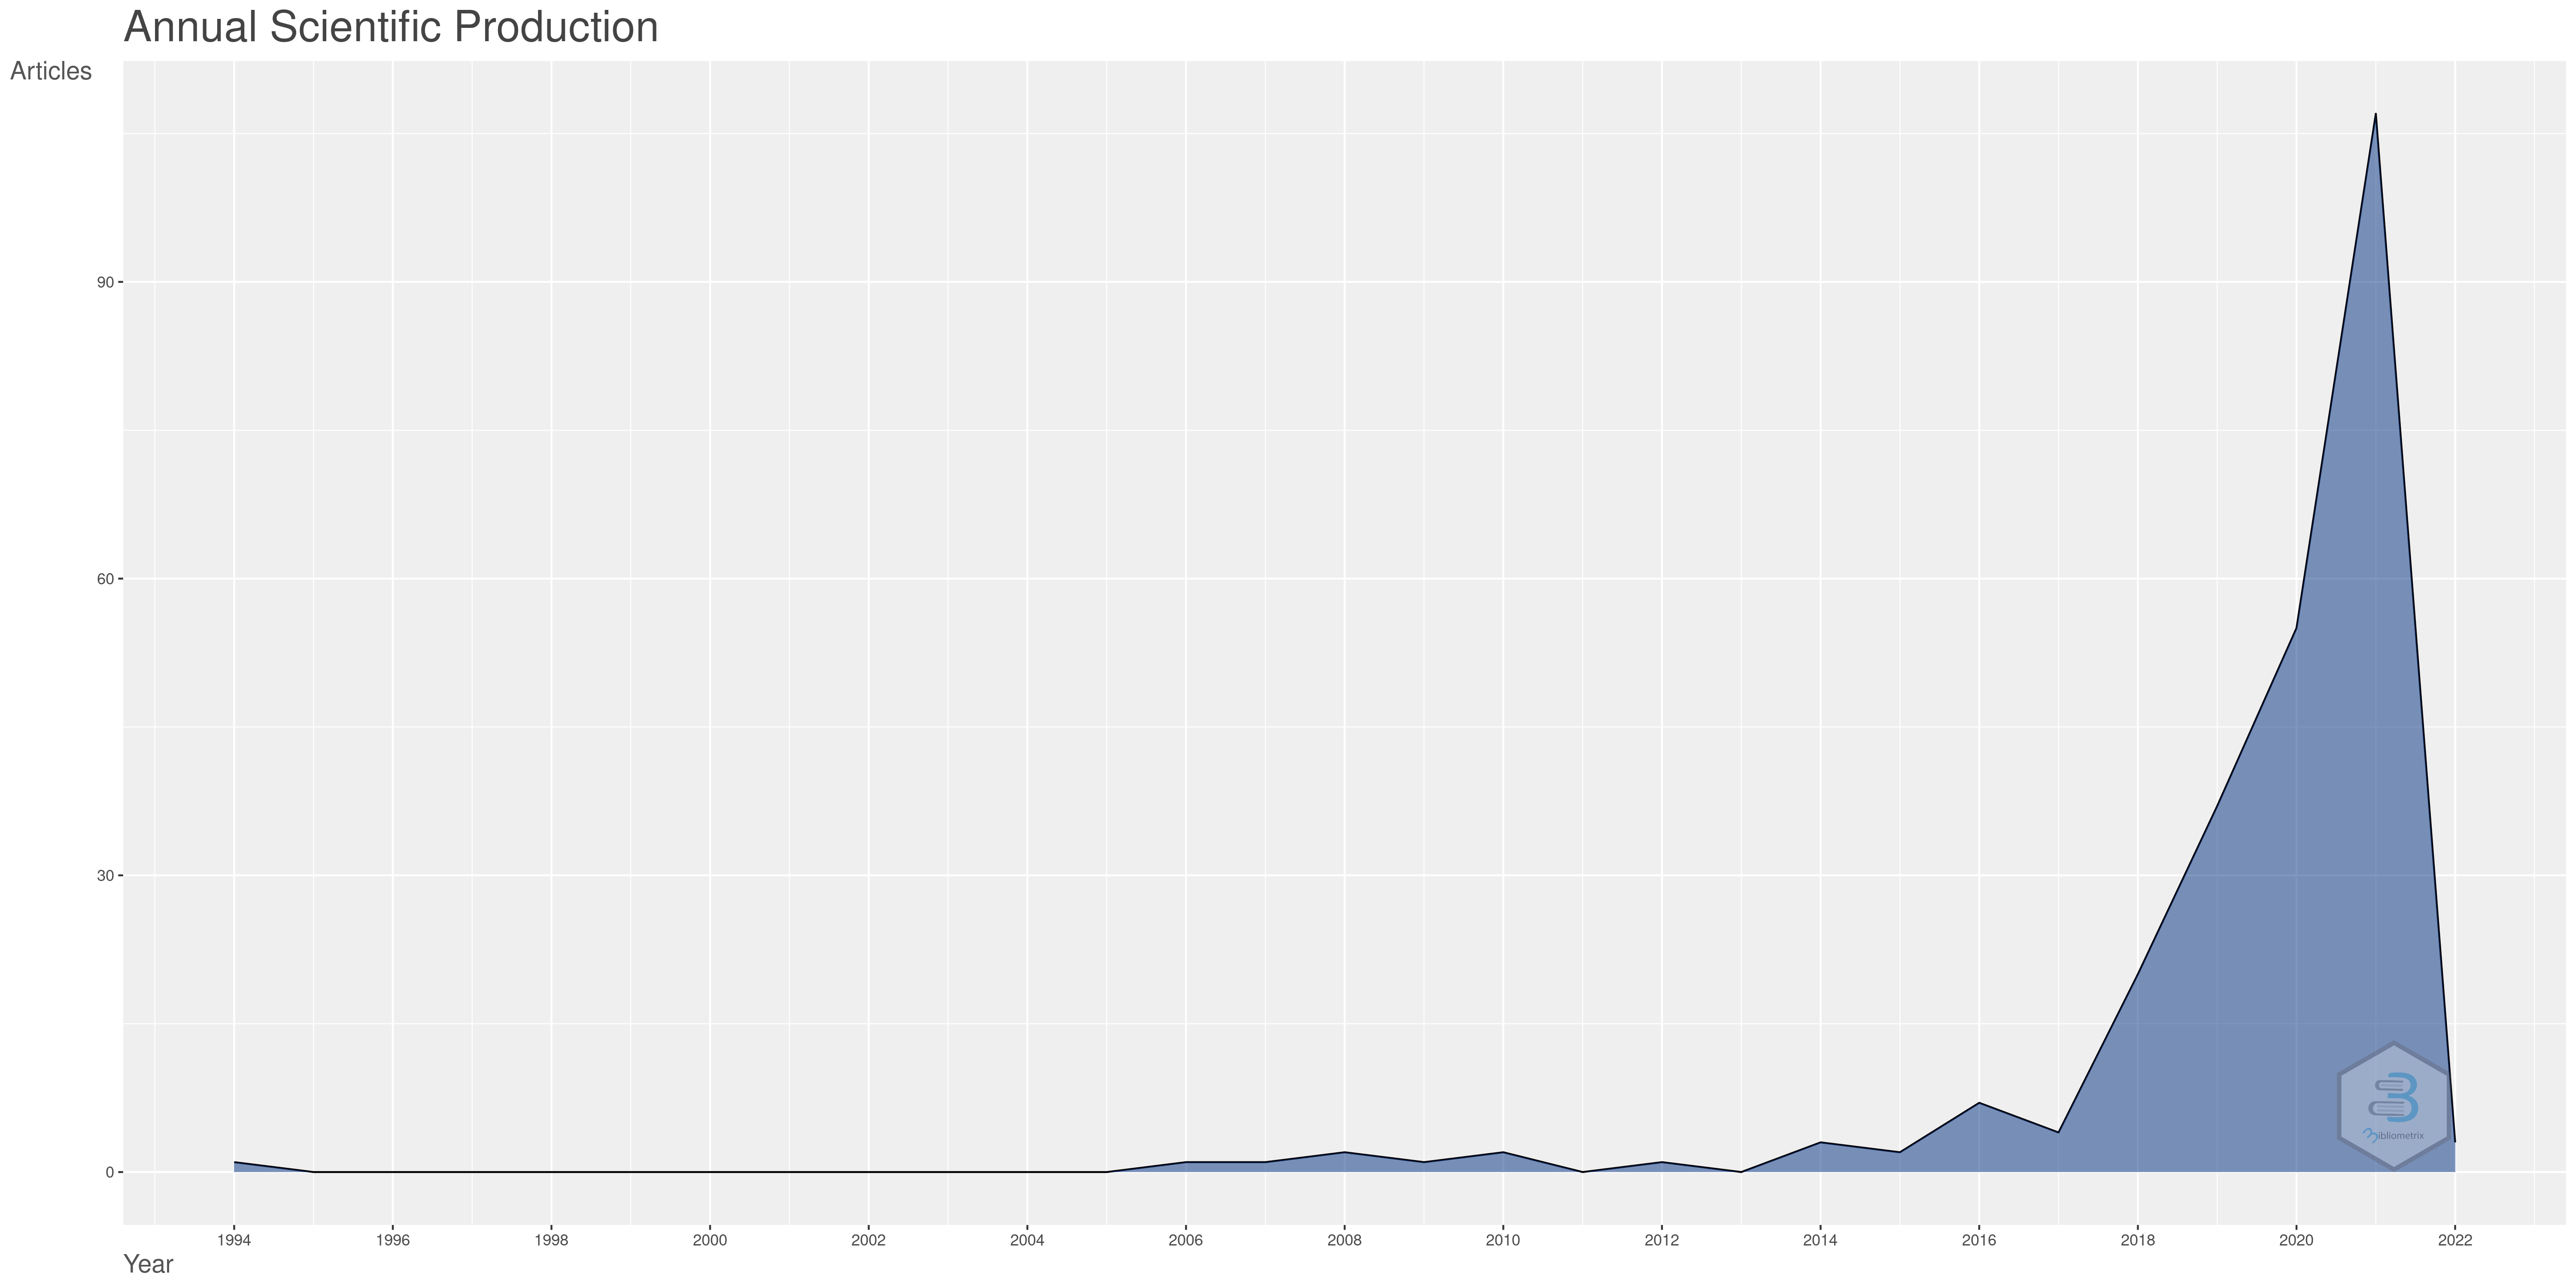
\includegraphics[width=1\textwidth]{experiments/gutorsantos/AnaliseBibliometrica/IAeDiscriminacao/imgs/AnnualScientificProduction-2022-02-09.png}
    \caption{Evolução da produção científica no dataset IADR@gutorsantos.}
    \label{fig:evol:anual:IADR@gutorsantos}
\end{figure}

Ao observar a figura \ref{fig:evol:anual:IADR@gutorsantos}, nota-se que nos anos iniciais do conjunto de dados (1994), não haviam pesquisas acerca do tema. A partir do meio do gráfico é quando se nota um crescente produção científica entorno do assunto. Vemos também que o gráfico se aproxima de uma forma exponencial. 
apresenta a evolução da produção científica mundial no tema de interesse. A curva mostra uma tendência de crescimento aproximadamente exponencial da quantidade de publicações, desde a primeira identificada em 1990.

O \textit{Annual Growth Rate} do dataset é de 7,6\%, ligeiramente maior que a taxa média de crescimento da publicação científica mundial, de cerca de 3,3\% anuais, em 2016, como ilustra o estudo em \url{https://www.researchgate.net/publication/333972683_Dynamics_of_scientific_production_in_the_world_in_Europe_and_in_France_2000-2016}, página 23.\footnote{Observa-se uma grande queda de 2021 para 2022 pois este estudo está sendo realizado no primeiro bimestre de 2022.}

\subsubsection{Interpretação do Crescimento} 

O Índice de Crescimento Anual indica que na última década assunto em pauta tem despertado interesse ainda que moderado. Porém esse índice aliado ao tamanho total do dataset (\totalDocuments{}) indica a importância de ressaltar a carência de pesquisadores e produções científicas nessa área. Apesar de uma taxa de crescimento não muito elevada, visualizamos por meio do gráfico que a curva tem uma tendência exponencial agressiva (veja a inclinação do gráfico nos anos de 2017 a 2021). Portanto, espera-se que nos próximos anos essa problemática seja resolvida parcialmente havendo um aumento substancial desse tema dentro do meio acadêmico.

\subsection{Evolução das Citações}
\label{sec:IADR@gutorsantos:Citations}

\begin{figure}[!h]
    \centering
    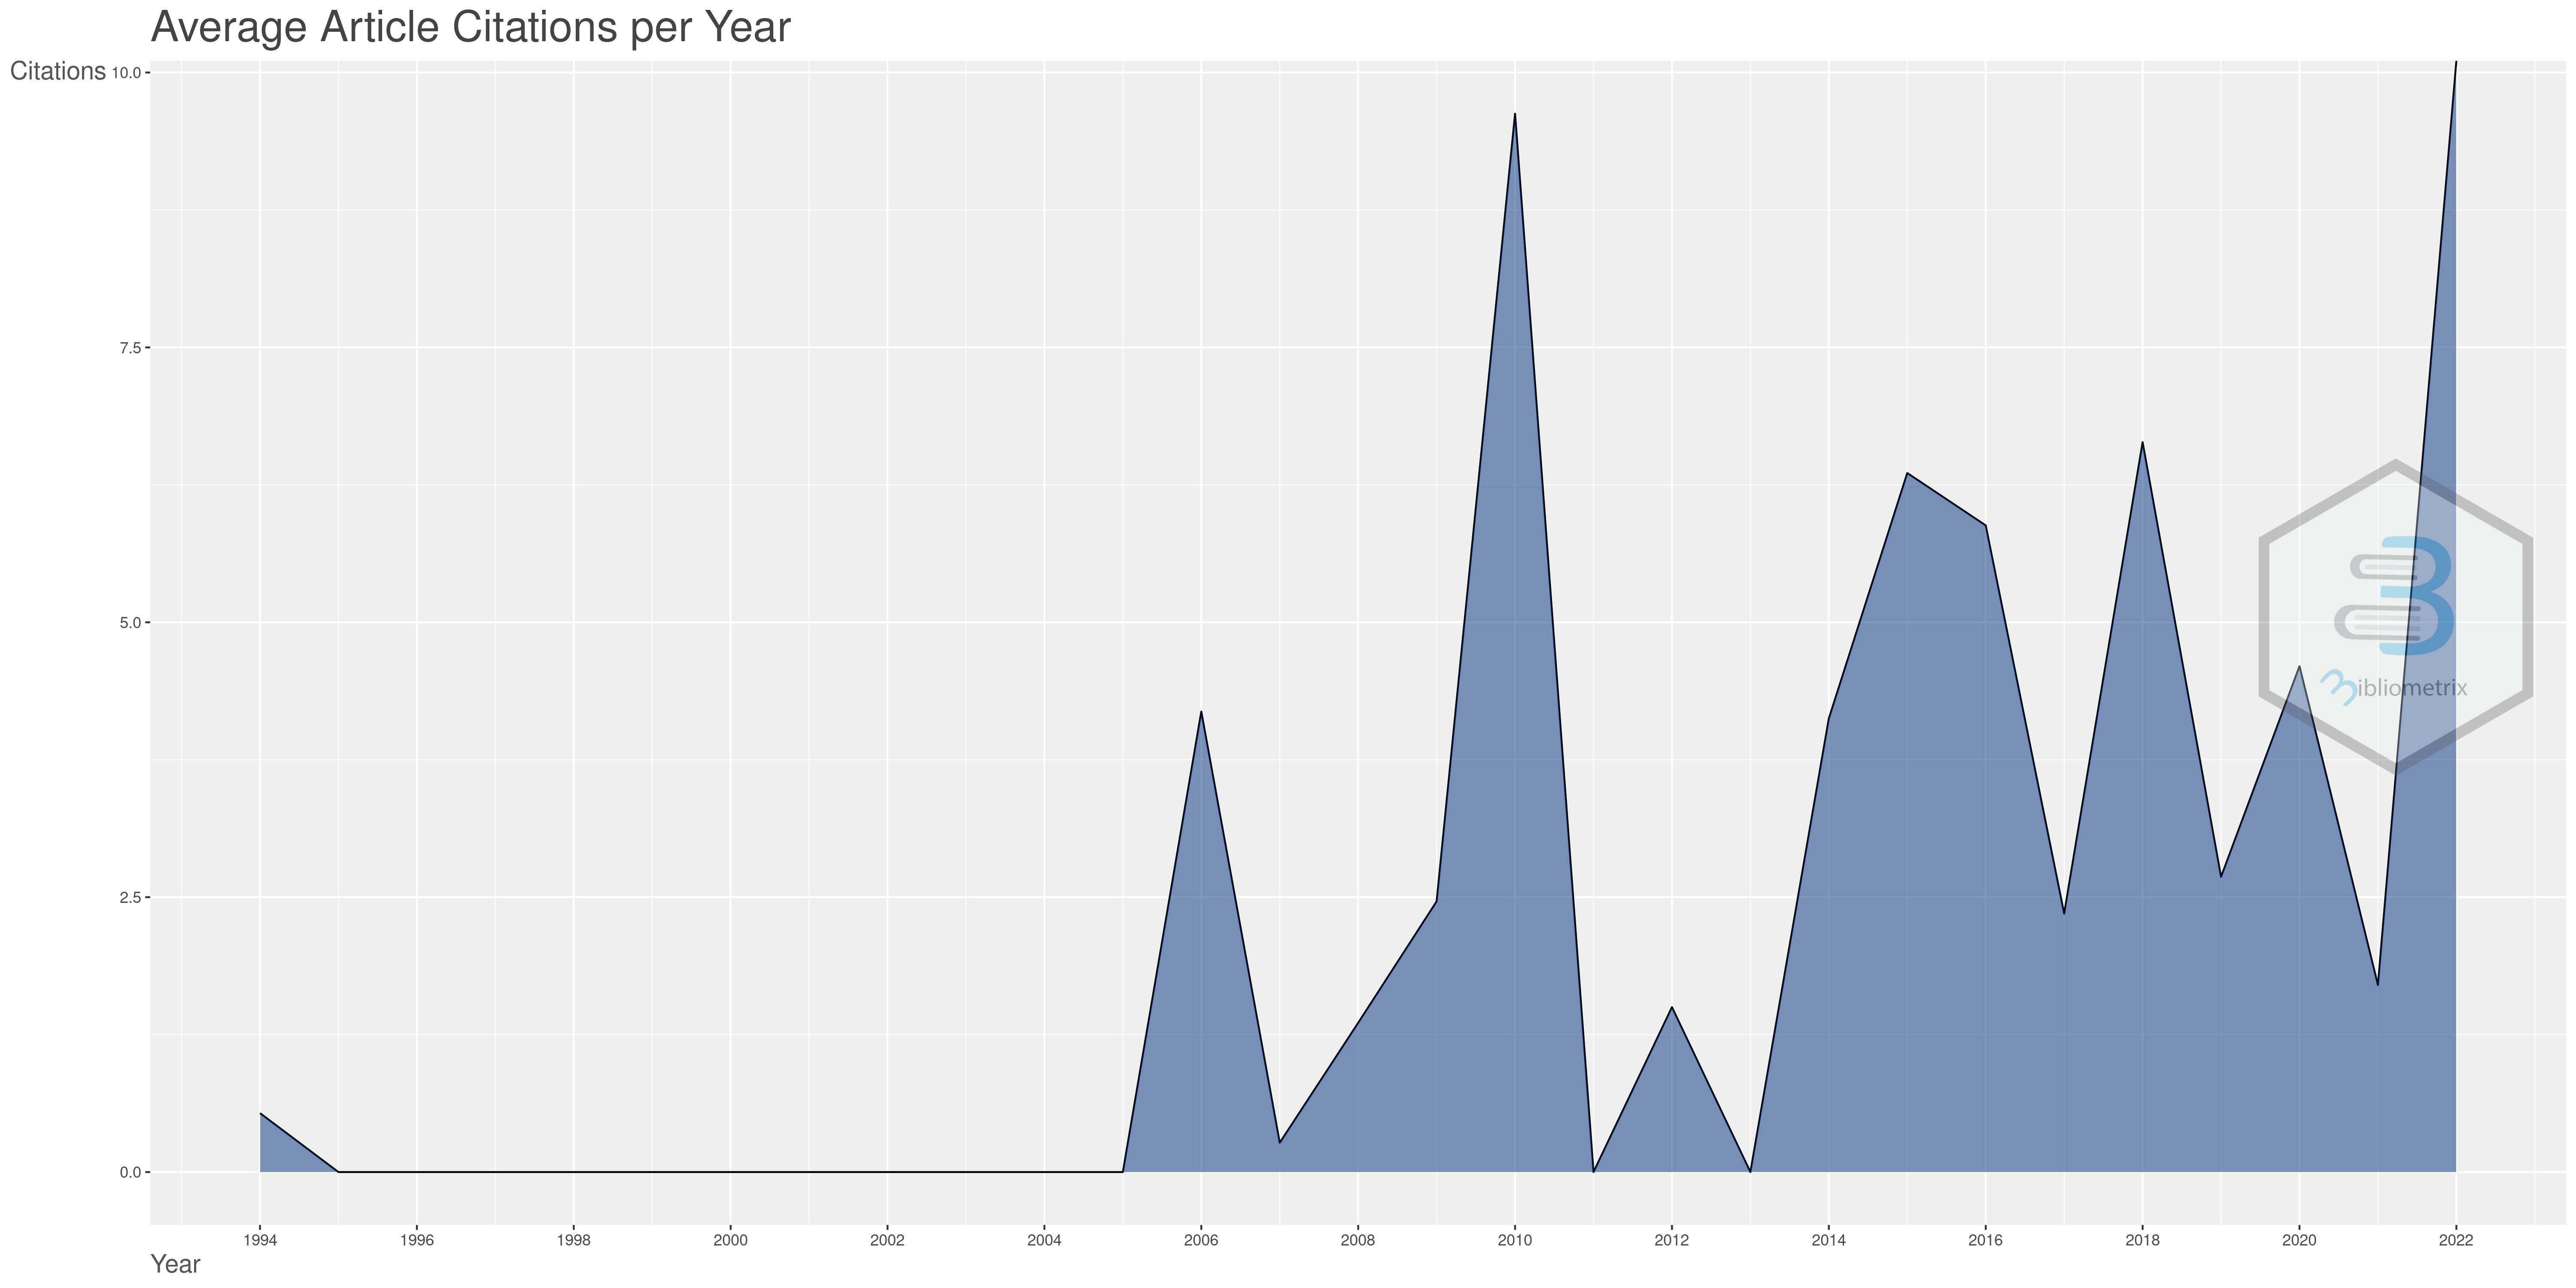
\includegraphics[width=1\textwidth]{experiments/gutorsantos/AnaliseBibliometrica/IAeDiscriminacao/imgs/AverageArticleCitationPerYear-2022-02-09.png}
    \caption{Evolução das citações ao dataset IADR@gutorsantos.}
    \label{fig:evol:anual:citacoes:IADR@gutorsantos}
\end{figure}

A figura \ref{fig:evol:anual:citacoes:IADR@gutorsantos} apresenta a evolução da média de citações aos \totalDocuments{} artigos no dataset IADR@gutorsantos. 
É possível notar uma grande variação na média ao longo dos anos. Entretanto há um pico que aparece no ano de 2010, isso se dá por causa da presença de uma artigo publicado em 2010, que é citado múltiplas vezes. Especificaremos adiante qual o artigo em questão.\footnote{Note que o cálculo do número  médio de citações, nesse caso, utiliza os valores computados no tag "TC (Times Cited)", já presentes no dataset obtido. Ou seja, o gráfico baseia-se no número de citações globais (externas ao dataset IADR@gutorsantos), e não no número de citações locais (citações a um artigo do dataset feitas por alguns dos outros artigos dentro do próprio dataset).}.

\subsubsection{Interpretação das Citações}
Apesar do crescimento exponencial da produção científica e da instabilidade na média de citações, é visível o leve crescimento nas citações médias ao longo dos anos sugere que os artigos do dataset possuem uma tendência de crescimento no tamanho da bibliografia citada, bem como também despertam grande interesse dos cientistas nas demais áreas do conhecimento (já que se trata de citações globais).

\subsection{\textit{Plotagem de Três Campos (Diagrama de Sankey)}}

O \textit{Three-Field Plots (Plotagem de Três Campos)} tem como objetivo mostrar os principais fluxos entre diferentes conjuntos de itens, desse modo, é evidenciado as correlações entre três conjuntos de atributos agregados que ocorrem no dataset.

\begin{figure}[!h]
    \centering
    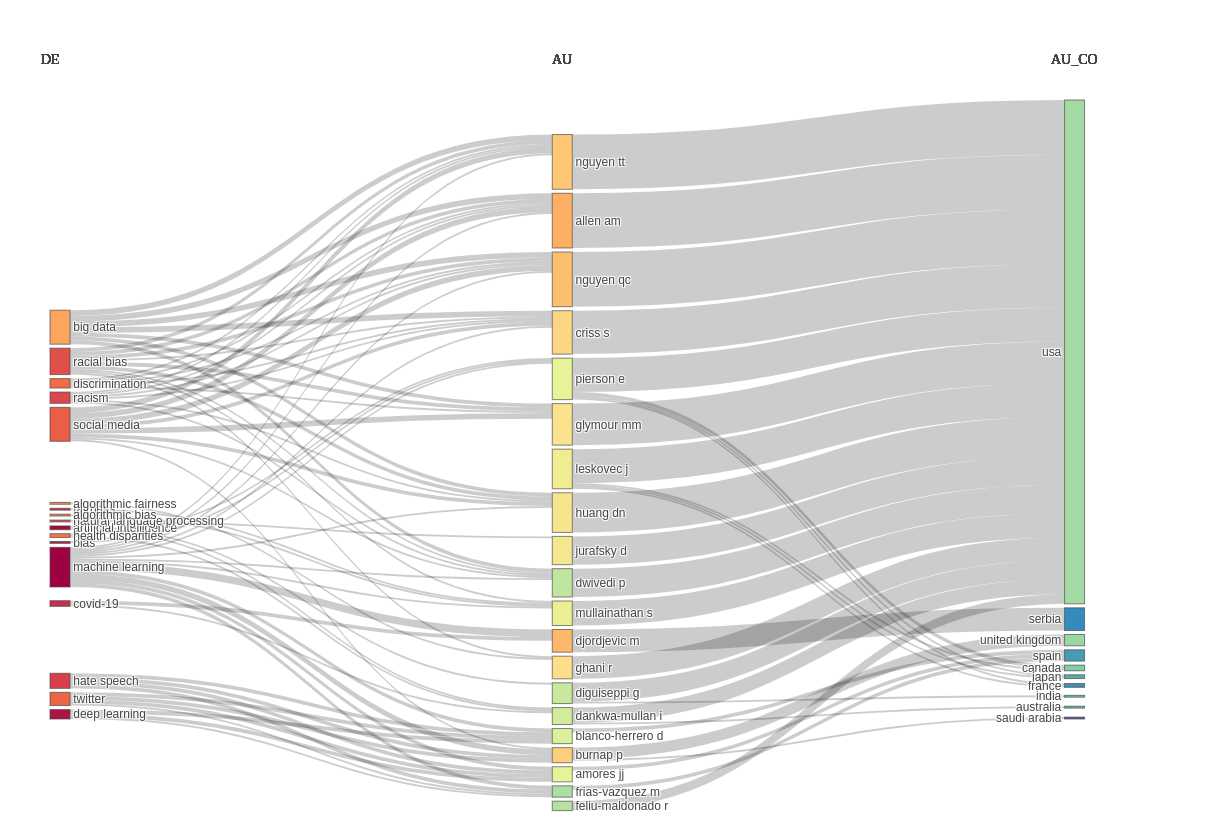
\includegraphics[angle=0,width=1\textwidth]{experiments/gutorsantos/AnaliseBibliometrica/IAeDiscriminacao/imgs/ThreeFieldPlot.png}
    \caption{Plotagem ``Três Campos'' (Sankey plot) do dataset IADR@gutorsantos: 20 Autores, Países e Palavras-Chave mais proeminentes.}
    \label{fig:IADR@gutorsantos:ThreeFieldPlot}
\end{figure}

A figura \ref{fig:IADR@gutorsantos:ThreeFieldPlot} apresenta a plotagem do tipo ``Três Campos'' do dataset MASSA@jhcf, vinculando, ao centro, os 20 Autores mais proeminentes (AU), à esquerda, as 20 Palavras-Chave de authores mais frequentes, e à direita, os 20 países proeminentes onde foram realizadas as pesquisas.

\subsubsection{Interpretação da figura \ref{fig:MASSA@jhcf:ThreeFieldPlot}}
Realizando a análise da direita para esquerda, vemos que há uma predominância dos Estados Unidos na produção científica do tema e que os principais autores realizaram suas pesquisas sediados em instituições deste mesmo país. Progredindo na análise é possível ver fluxos dos principais autores com as palavras-chaves mais frequentes e que mais possuem relação direta com os termos de busca.

Adicionalmente, dentre as palavras-chave (DE) não relacionadas diretamente aos termos de busca, emergem os termos \textbf{covid-19}, \textbf{hate speech}, \textbf{twitter}. A primeira, indica problemas de desigualdade na área de saúde possívelmente, especificamente no contexto da pandemia do Covid-19, sendo ligada ao tema central pela palavra-chave \textit{artificial intelligence}, sugerindo que possa estar ocorrendo um quadro de discriminação na área médica através do uso de Inteligência Artificial. As outras duas palavras estão ligadas à tentativa de identificar discursos de ódio em redes sociais, como o twitter, utilizando técnicas baseadas em IA.

\subsection{Análises Bibliométricas: Fontes de Informação}

Para a análise acerca das Fontes de Informação, nos valeremos das seguintes três imagens.

\begin{figure}[!h]
    \centering
    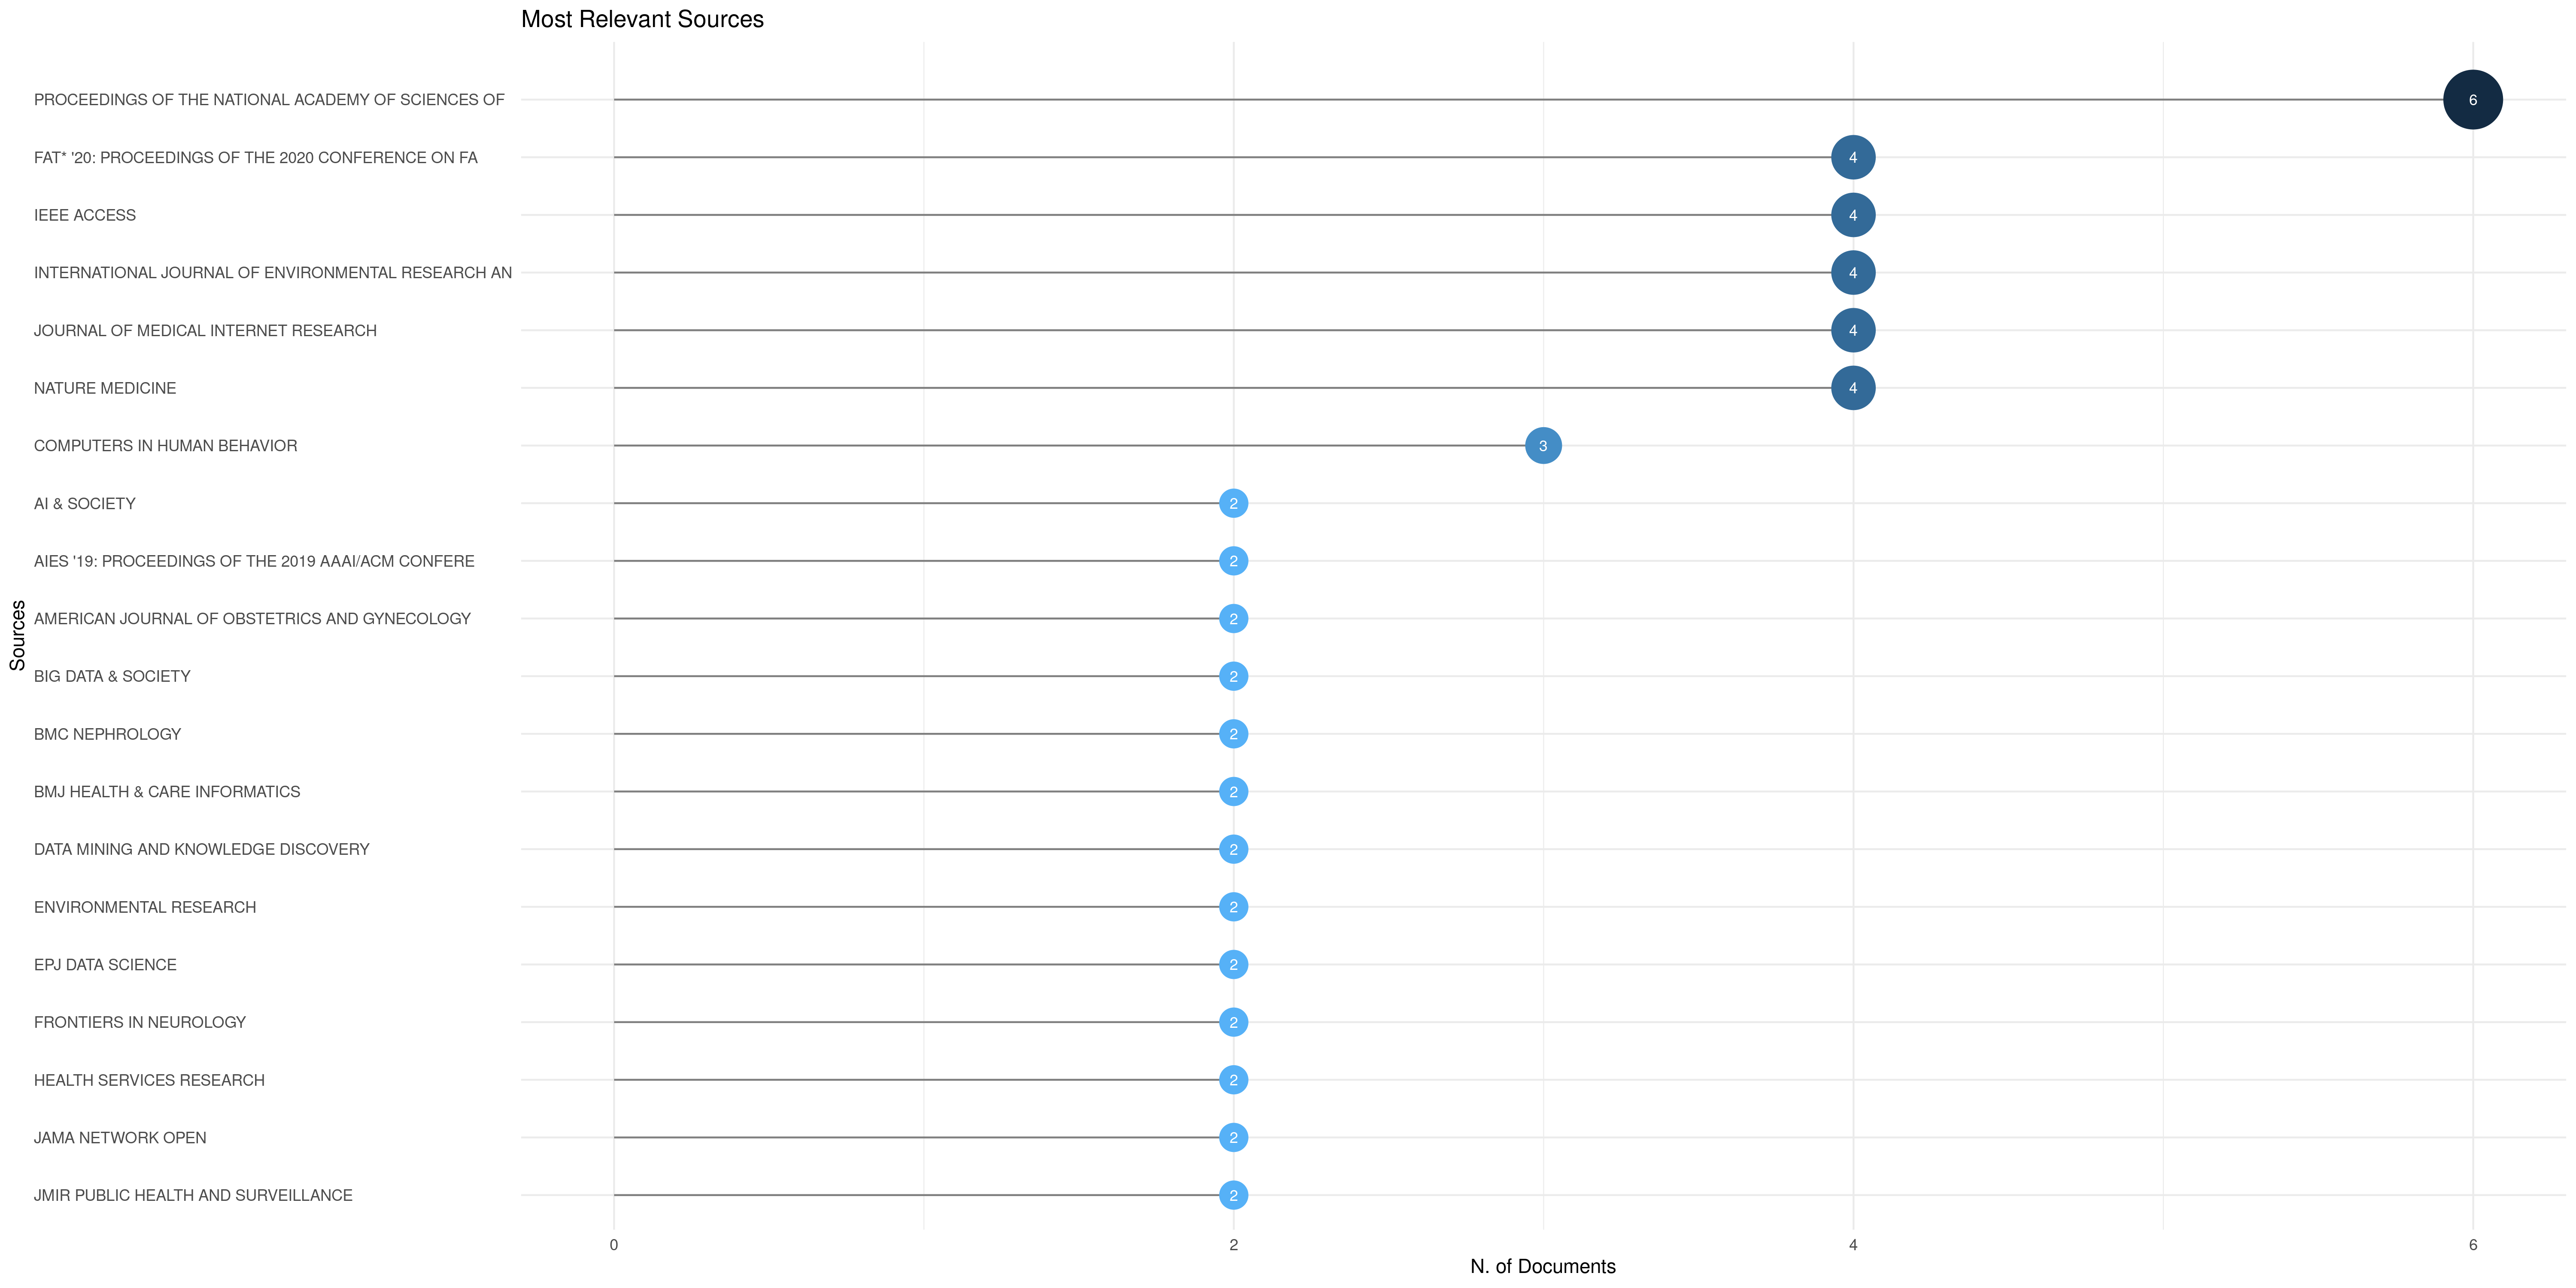
\includegraphics[angle=0,width=1\textwidth]{experiments/gutorsantos/AnaliseBibliometrica/IAeDiscriminacao/imgs/MostRelevantSources-2022-02-09.png}
    \caption{Fontes de Informação mais Relevantes do dataset IADR@gutorsantos.}
    \label{fig:IADR@gutorsantos:RelevantSources}
\end{figure}

\begin{figure}[!h]
    \centering
    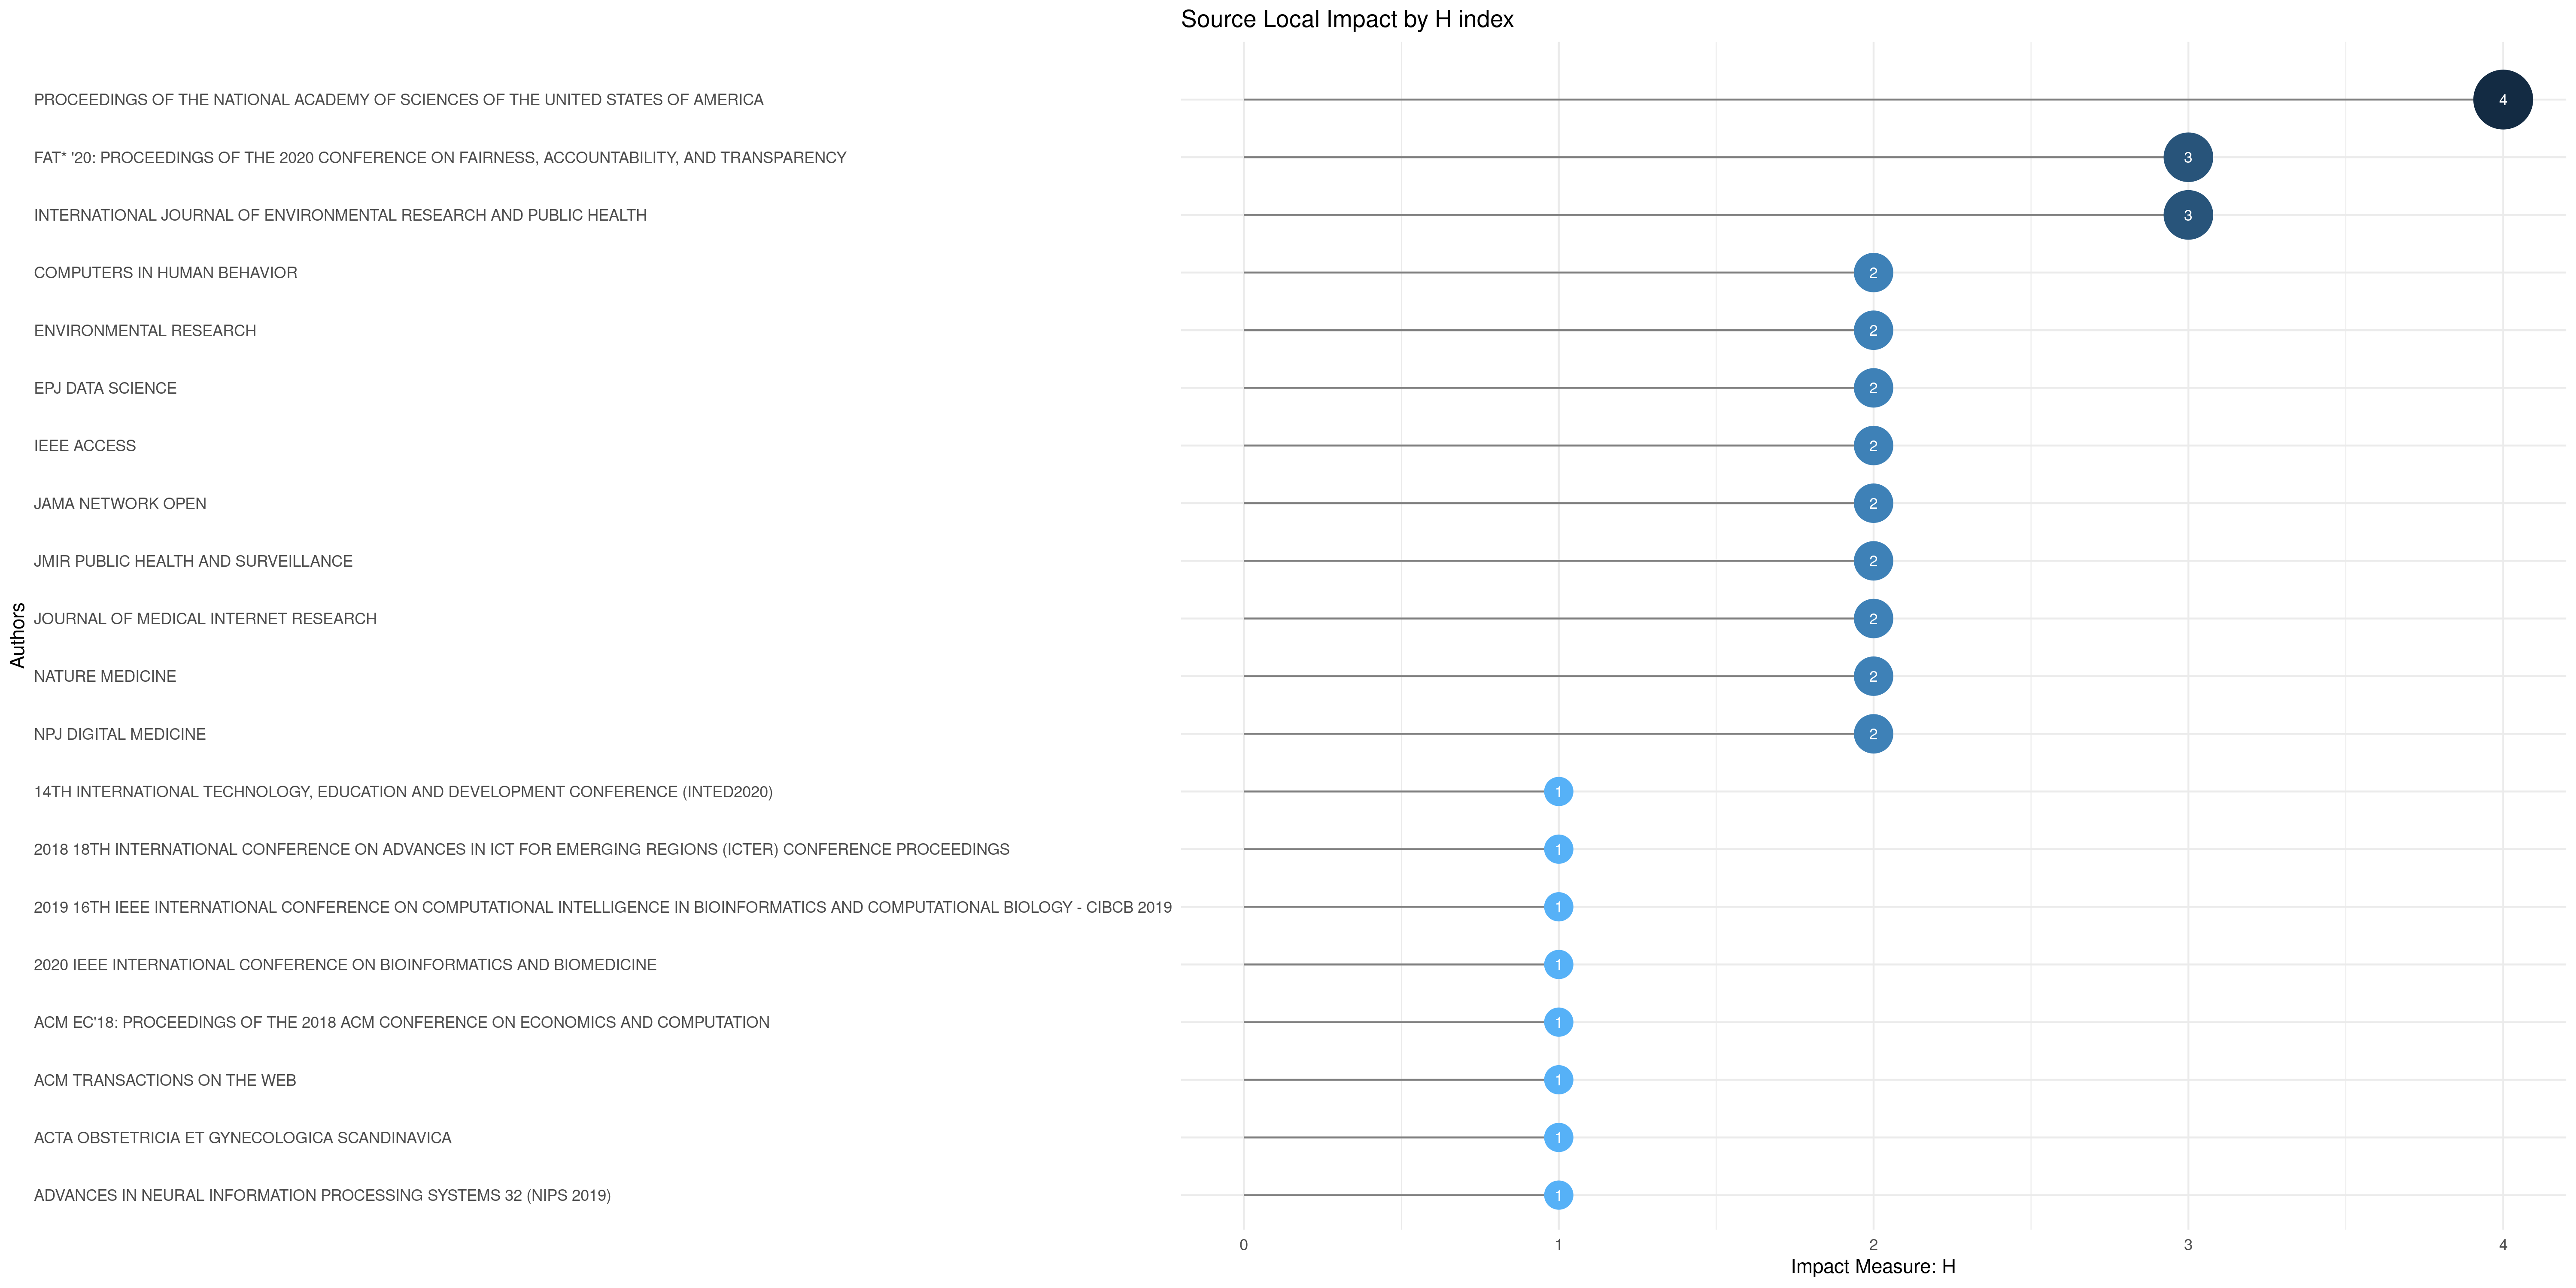
\includegraphics[angle=0,width=1\textwidth]{experiments/gutorsantos/AnaliseBibliometrica/IAeDiscriminacao/imgs/SourceImpact-2022-02-09.png}
    \caption{Impacto das Fontes de Informação no dataset IADR@gutorsantos.}
    \label{fig:IADR@gutorsantos:SourceImpact}
\end{figure}

\begin{figure}[!h]
    \centering
    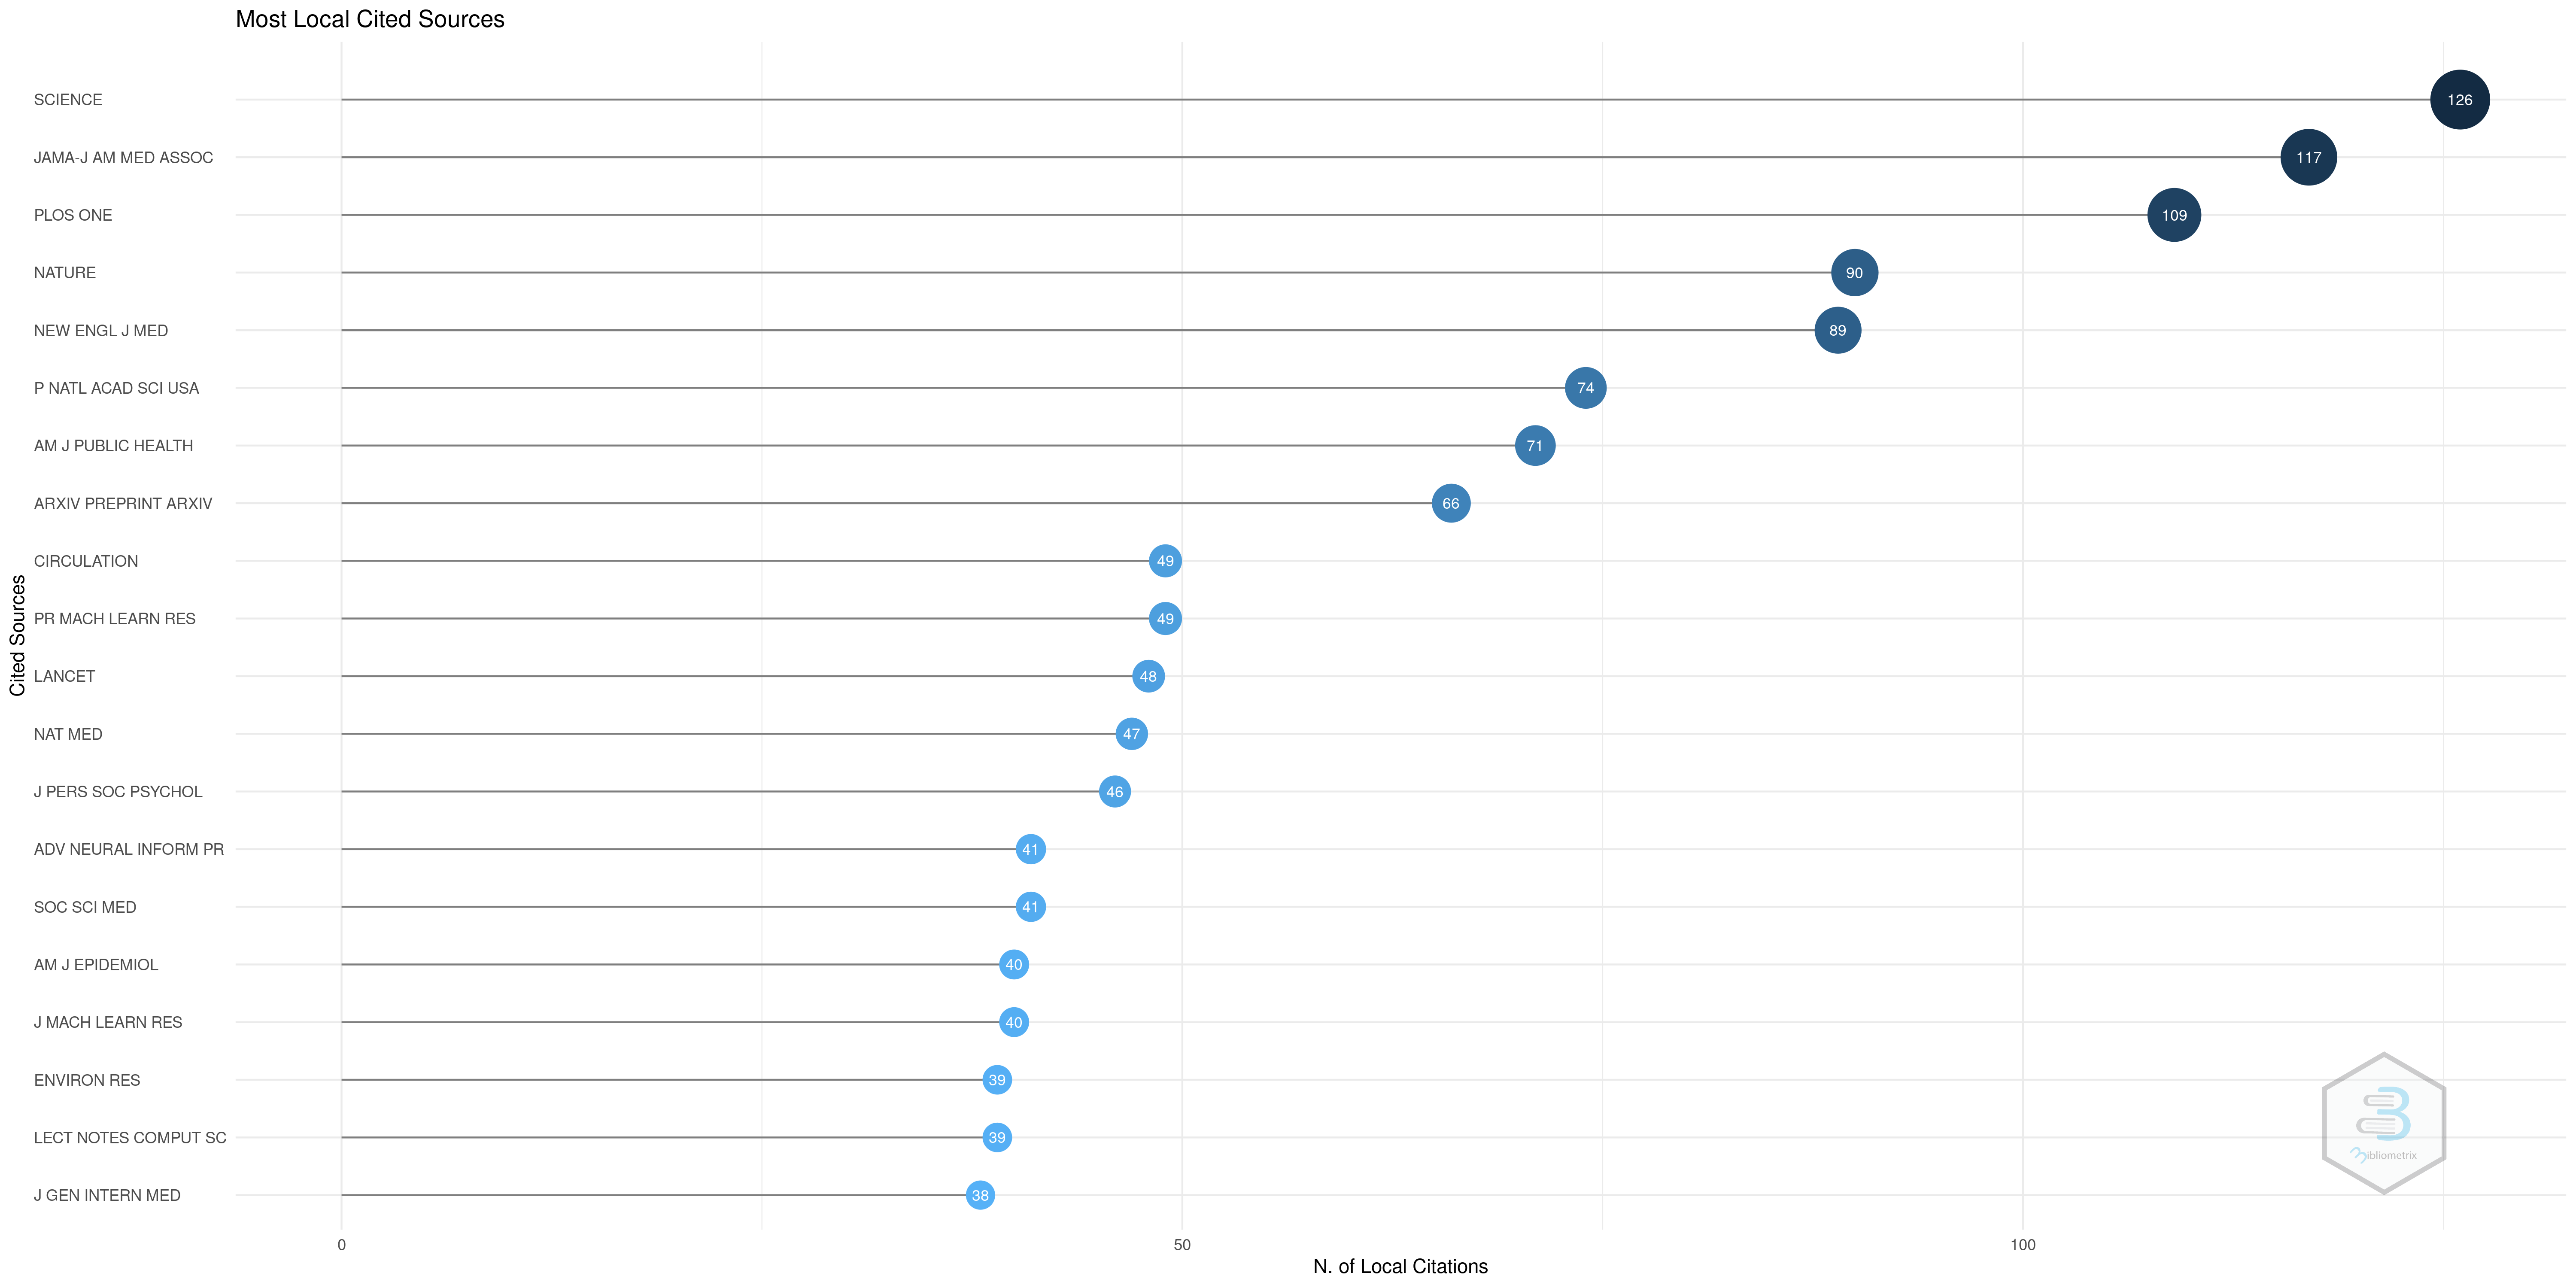
\includegraphics[angle=0,width=1\textwidth]{experiments/gutorsantos/AnaliseBibliometrica/IAeDiscriminacao/imgs/MostLocalCitedSources-2022-02-09.png}
    \caption{Fontes de Informação locais mais citadas do dataset IADR@gutorsantos.}
    \label{fig:IADR@gutorsantos:MostCitedSources}
\end{figure}

\subsubsection{Interpretação das figuras }
Vemos na figura \ref{fig:IADR@gutorsantos:SourceImpact} que grande parte dos artigos são publicados em fontes de cunho computacional porém vemos a presença de várias fontes relacionadas à área médica. Essas áreas se relacionam a medida que há estudos sobre patologias que podem ser desenvolvidas ou agravadas por estados psíquicos instáveis ocasionados pelos impactos da discriminação racial.

Entretanto ao analisar a figura podemos ver que essas fontes não possuem um impacto alto para os outros registros do conjunto de dados. Indicando a relação mas não a predominância. Sendo assim, o maior impacto causado pelas fontes relacionadas a computação e áreas correlatas.

Na figura \ref{fig:IADR@gutorsantos:MostCitedSources} observamos que nas fontes locais mais citadas, temos um grande quantidade de fontes médicas em meio as fontes da área de computação, isso indicada uma preocupação dos autores em relação à saúde dos indivíduos uma vez que estes estão sob influência negativa dos algoritmos de IA.

\subsection{Análises Bibliométricas: Autores}

Para a análise acerca dos Autores, devemos considerar as seguintes imagens abaixo.

\begin{figure}[!h]
    \centering
    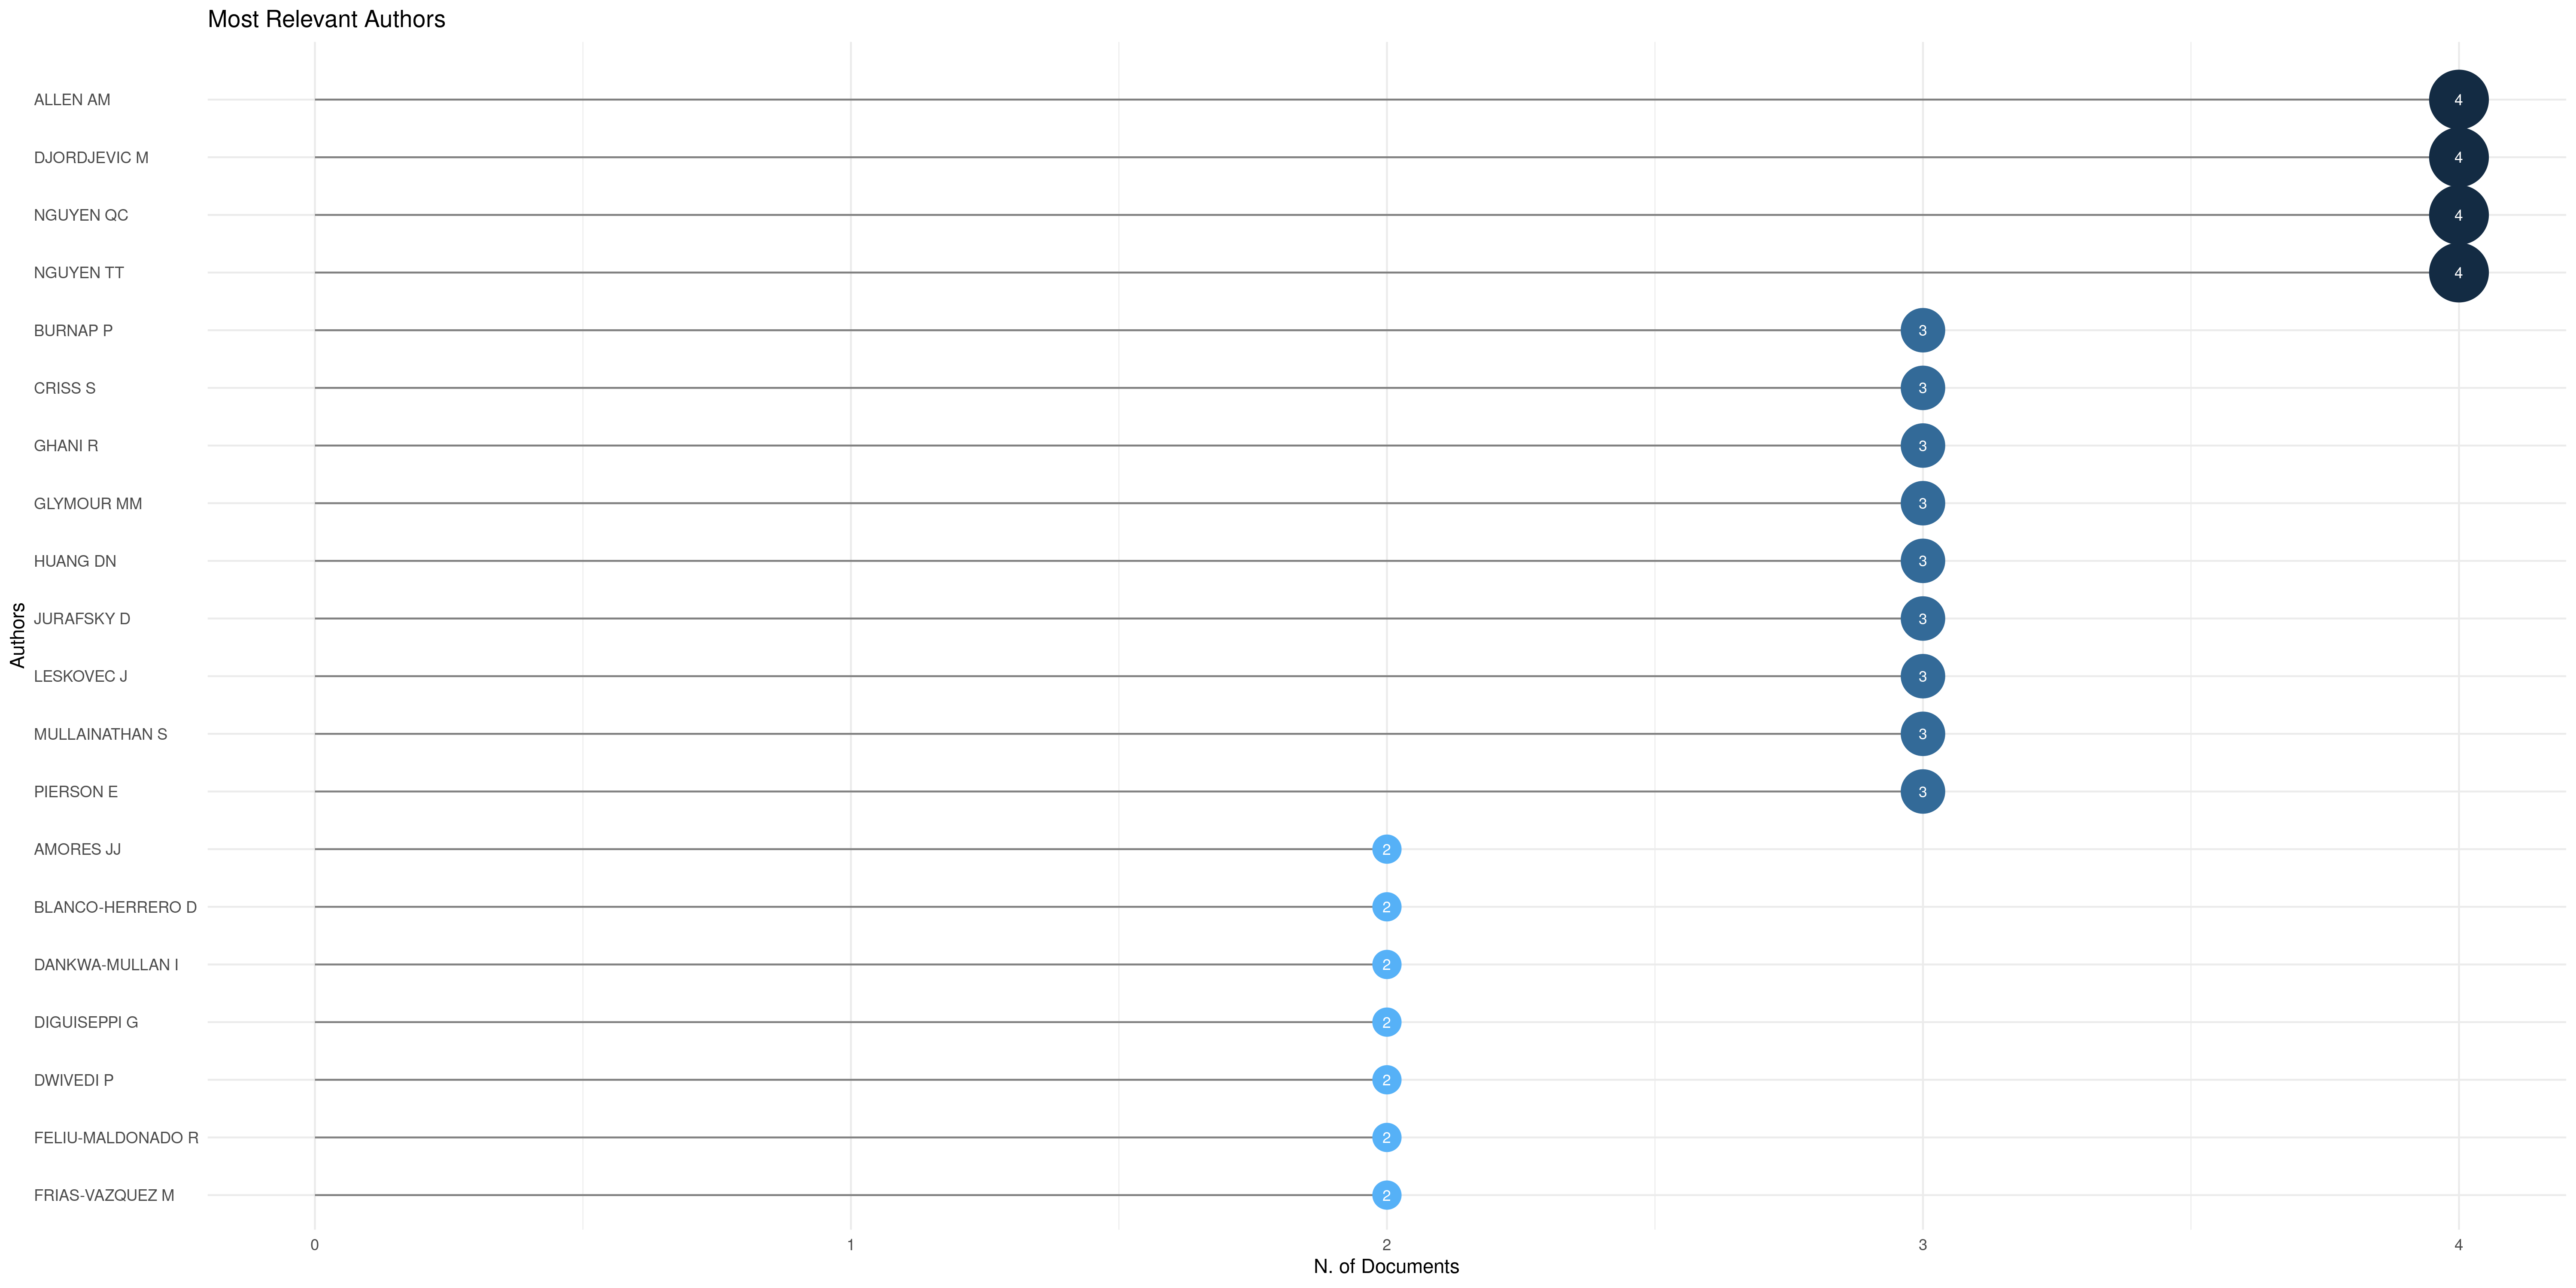
\includegraphics[angle=0,width=1\textwidth]{experiments/gutorsantos/AnaliseBibliometrica/IAeDiscriminacao/imgs/MostRelevantAuthors-2022-02-09.png}
    \caption{Autores relevantes do dataset IADR@gutorsantos.}
    \label{fig:IADR@gutorsantos:RelevantAuthors}
\end{figure}

\begin{figure}[!h]
    \centering
    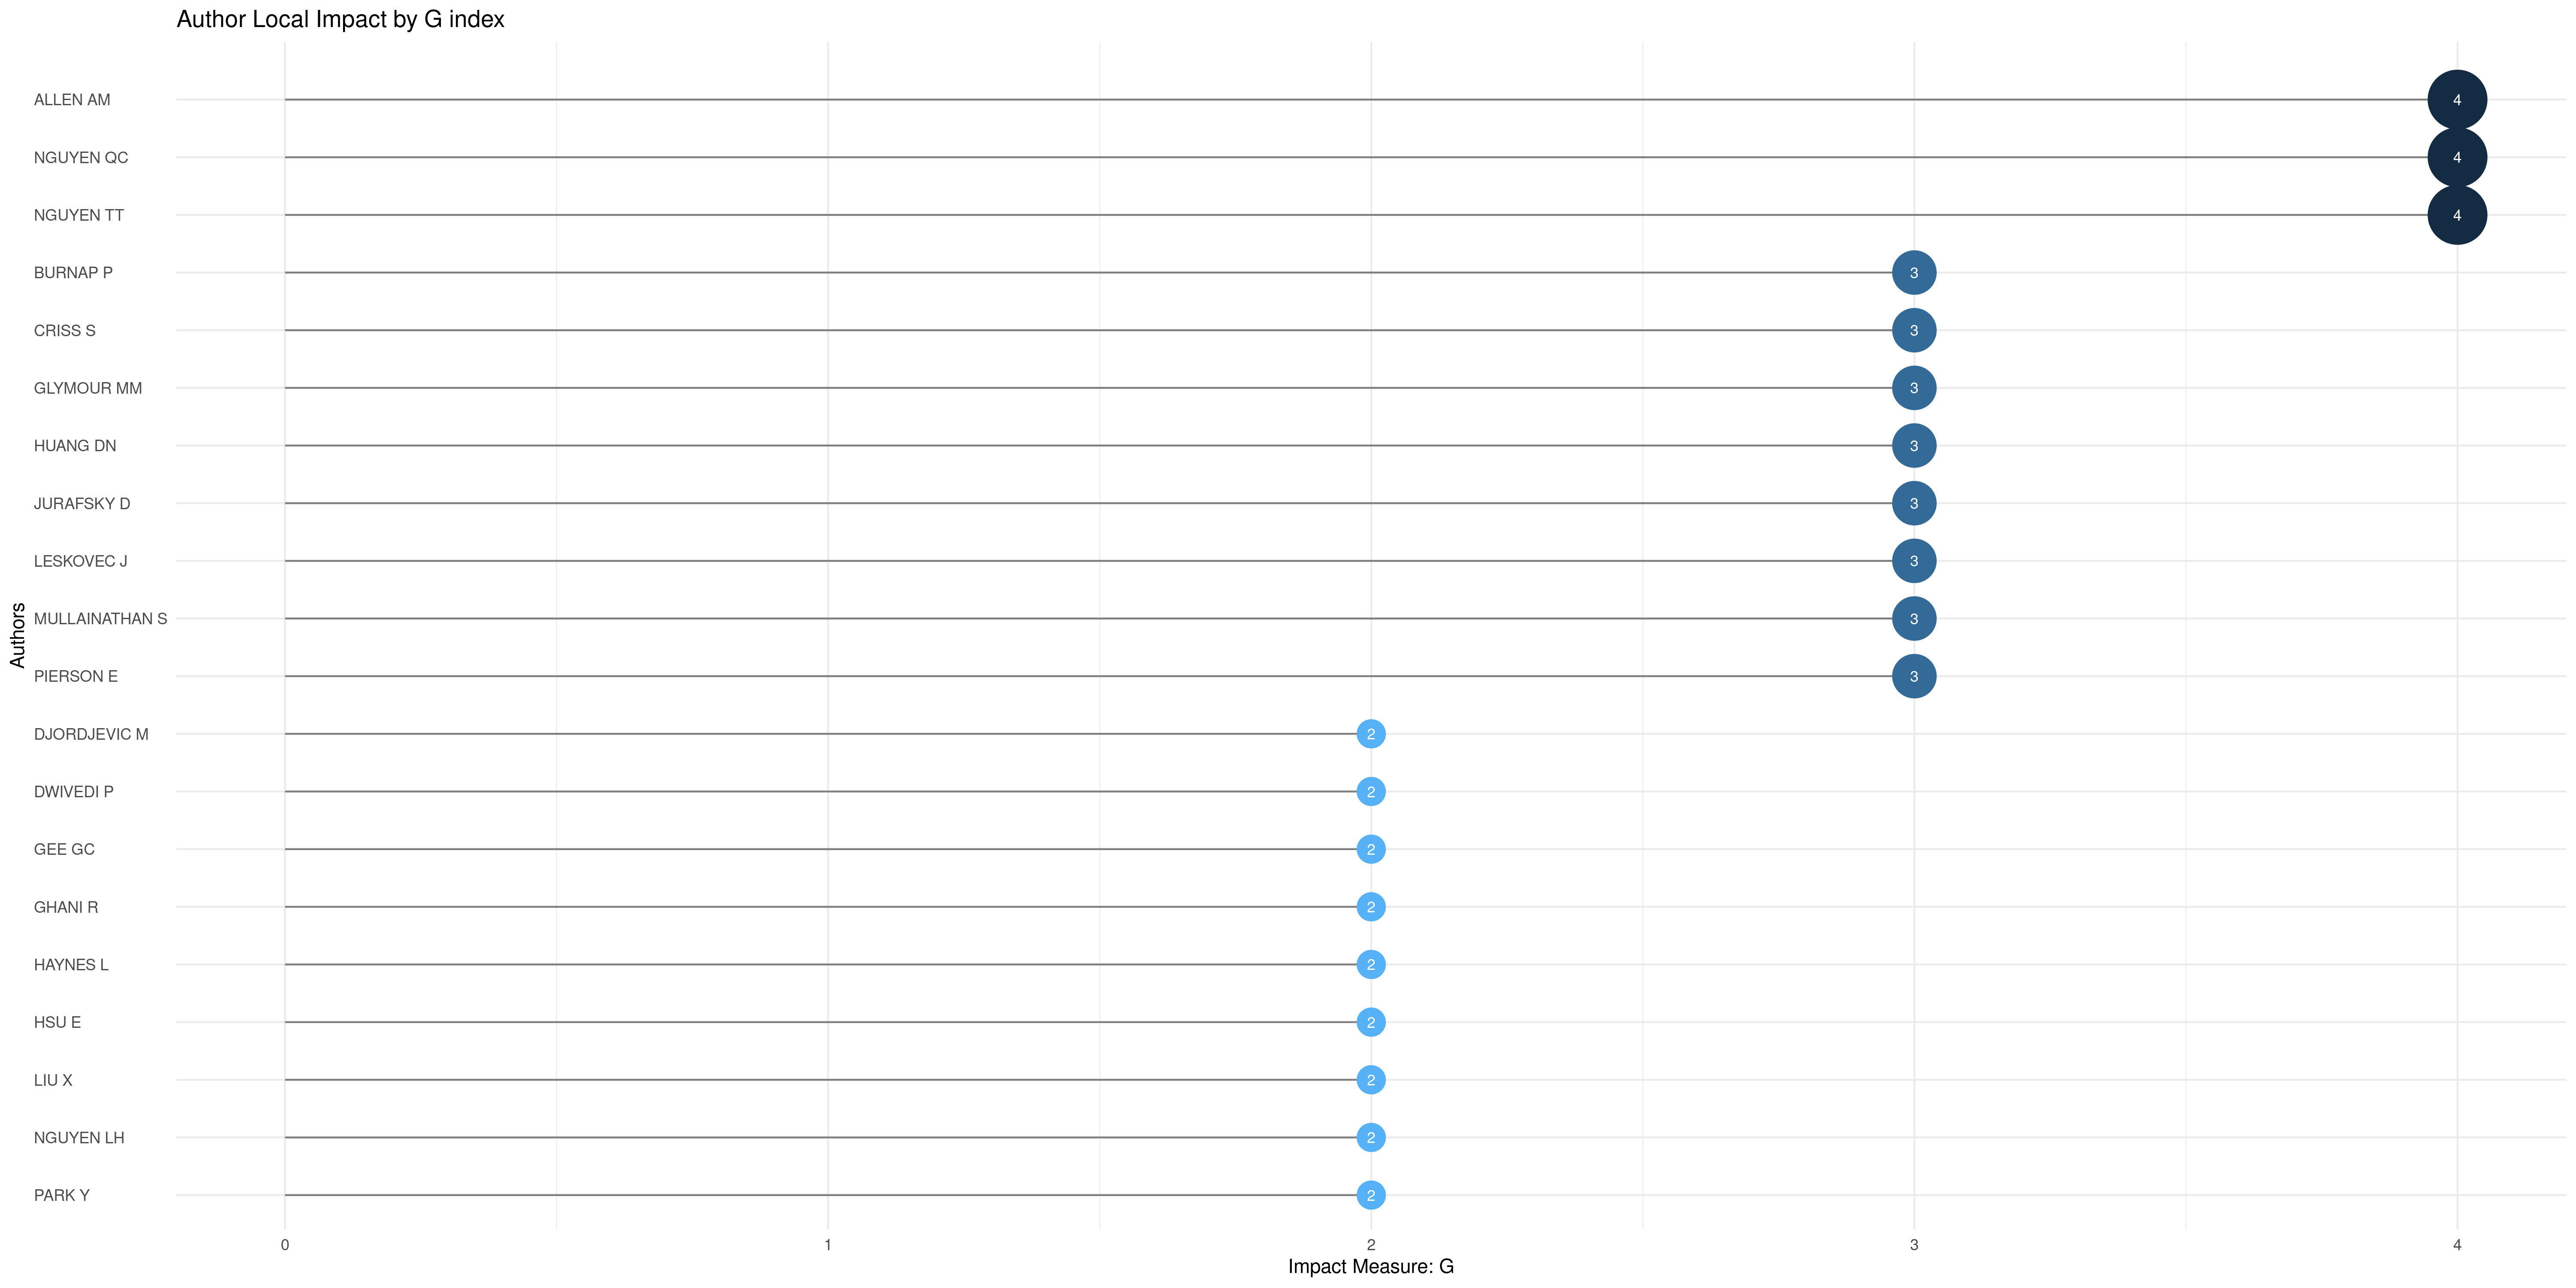
\includegraphics[angle=0,width=1\textwidth]{experiments/gutorsantos/AnaliseBibliometrica/IAeDiscriminacao/imgs/AuthorImpact-2022-02-09.png}
    \caption{Impacto dos Autores no dataset IADR@gutorsantos.}
    \label{fig:IADR@gutorsantos:AuthorsImpact}
\end{figure}

\begin{figure}[!h]
    \centering
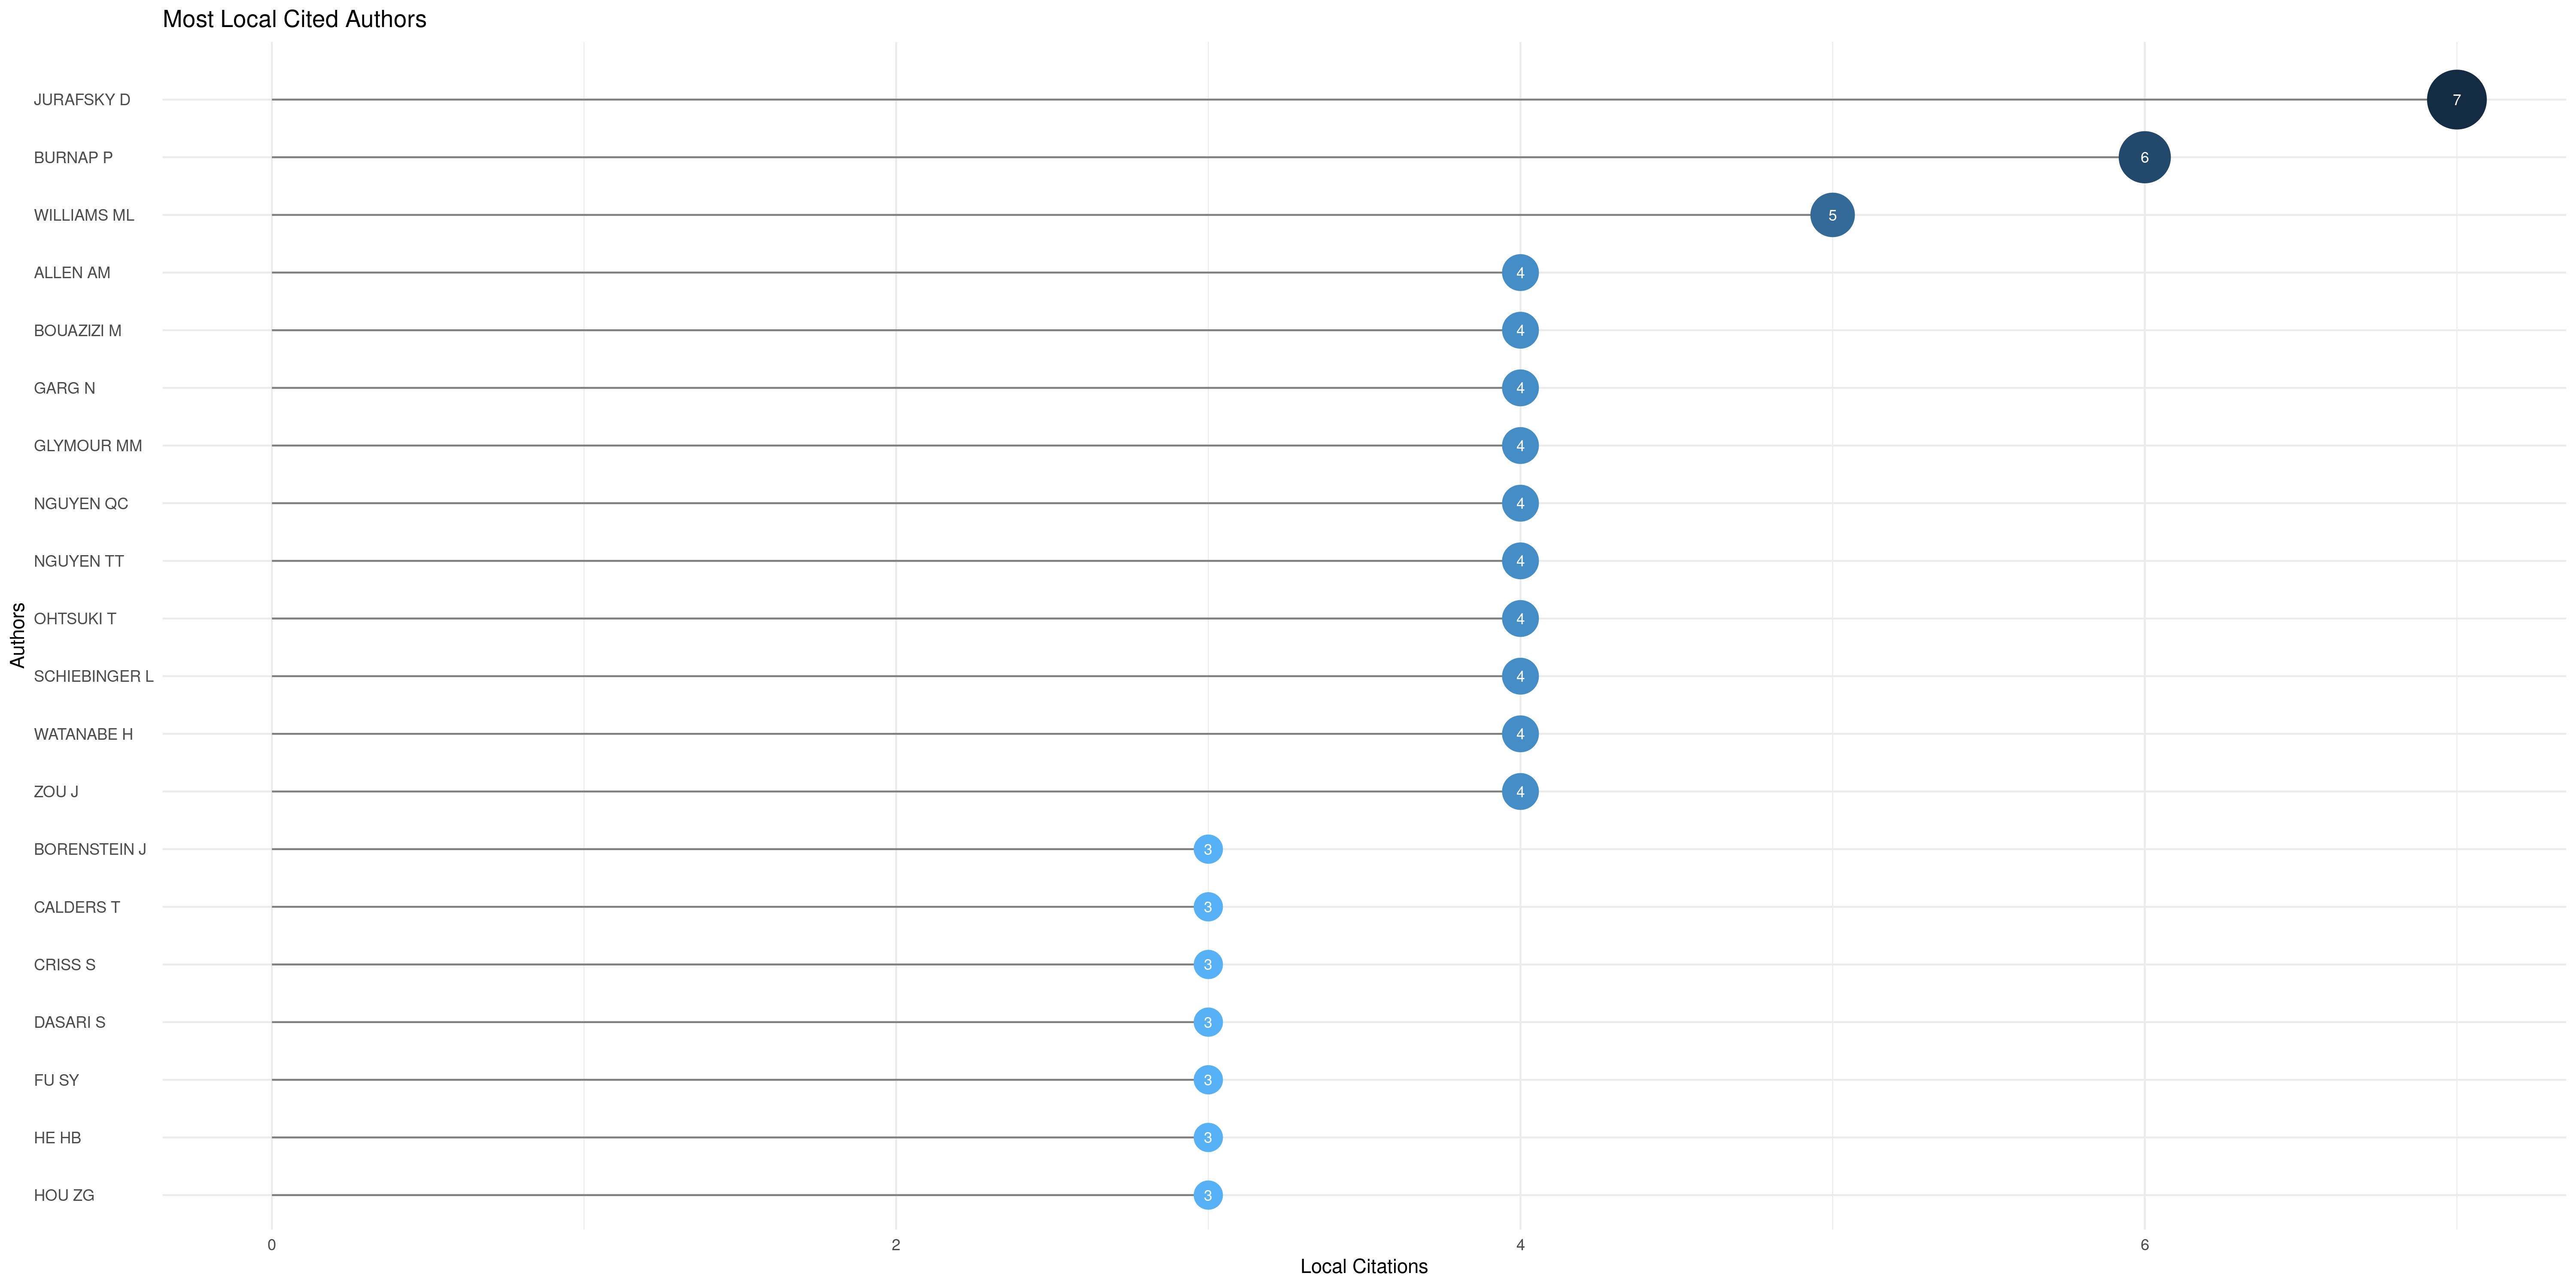
\includegraphics[angle=0,width=1\textwidth]{experiments/gutorsantos/AnaliseBibliometrica/IAeDiscriminacao/imgs/MostLocalCitedAuthors-2022-02-09.png}
    \caption{Autores locais mais citados do dataset IADR@gutorsantos.}
    \label{fig:IADR@gutorsantos:MostCitedAuthors}
\end{figure}

\begin{figure}[!h]
    \centering
    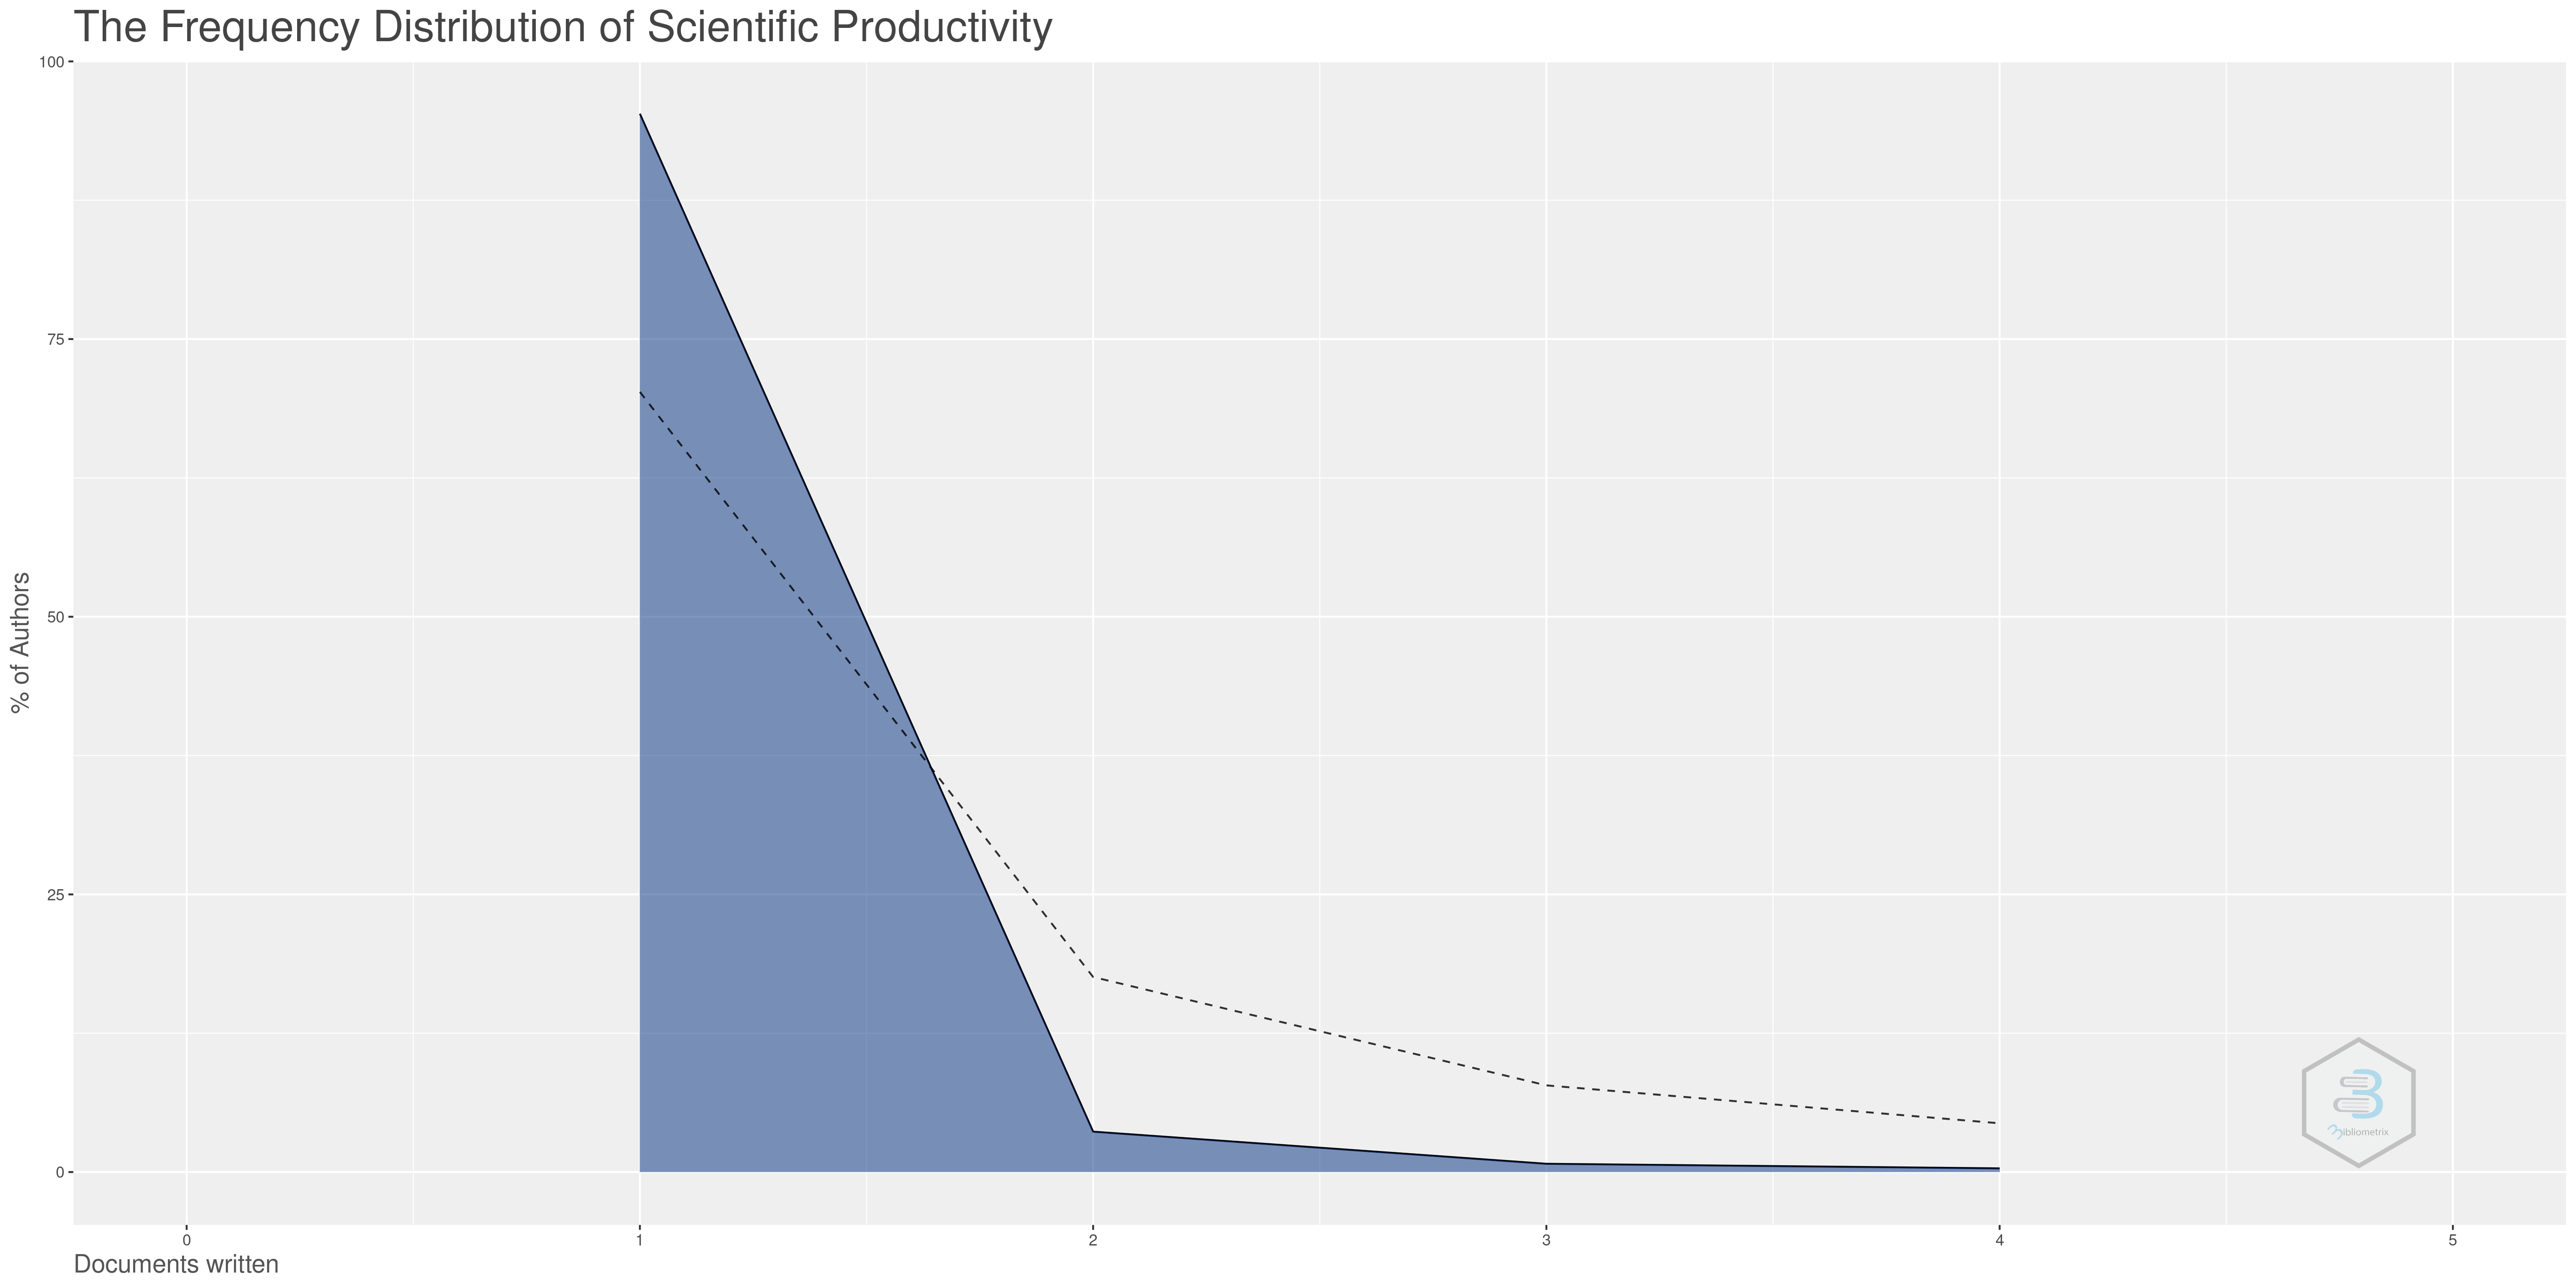
\includegraphics[angle=0,width=1\textwidth]{experiments/gutorsantos/AnaliseBibliometrica/IAeDiscriminacao/imgs/LotkaLaw-2022-02-09.png}
    \caption{Frequência de publição dos artigos dos Autores do dataset IADR@gutorsantos. (Lei de Lotka)}
    \label{fig:IADR@gutorsantos:Lotka}
\end{figure}

\subsubsection{Interpretação das figuras }
As figuras \ref{fig:IADR@gutorsantos:RelevantAuthors}, \ref{fig:IADR@gutorsantos:AuthorsImpact} e \ref{fig:IADR@gutorsantos:MostCitedAuthors} nos auxiliam a identificar os autores mais relevantes, os que mais influenciam e quais são os mais citado dentro do própio conjunto de dados.

Entretanto, considerando a figura \ref{fig:IADR@gutorsantos:Lotka} podemos ver que quase 100\% dos autores possuem apenas um artigo referente ao tema, consequentemente, não há continuação da pesquisa nessa área --- basta ver a drástica queda na porcentagem de autores que possuem um para dois artigos. Desse modo, tomando em consideração a curva pontilhada, vemos que as publicações referentes ao assunto estão consideravelmente fora do padrão esperado. Tendo isso em vista, há uma perda na qualidade da produção científica pois não ocorre o aprofundamento nesse campo o que dificulta o desenvolvimento de bons artigos de referência.


\subsection{Análises Bibliométricas: Documentos}

Para enriquecer a compreensão da análise acerca dos documentos, primeiro devemos identificar quais são os artigos mais citados globalmente --- não necessariamente estão presentes nesse conjunto de dados -- quais são artigos mais citados dentro do próprio dataset. Portanto, as figuras \ref{fig:IADR@gutorsantos:GlobalCitedDocs} e \ref{fig:IADR@gutorsantos:LocalCitedDocs}, abaixo, nos ajudam a verificar esses parâmetros.

\begin{figure}[!h]
    \centering
    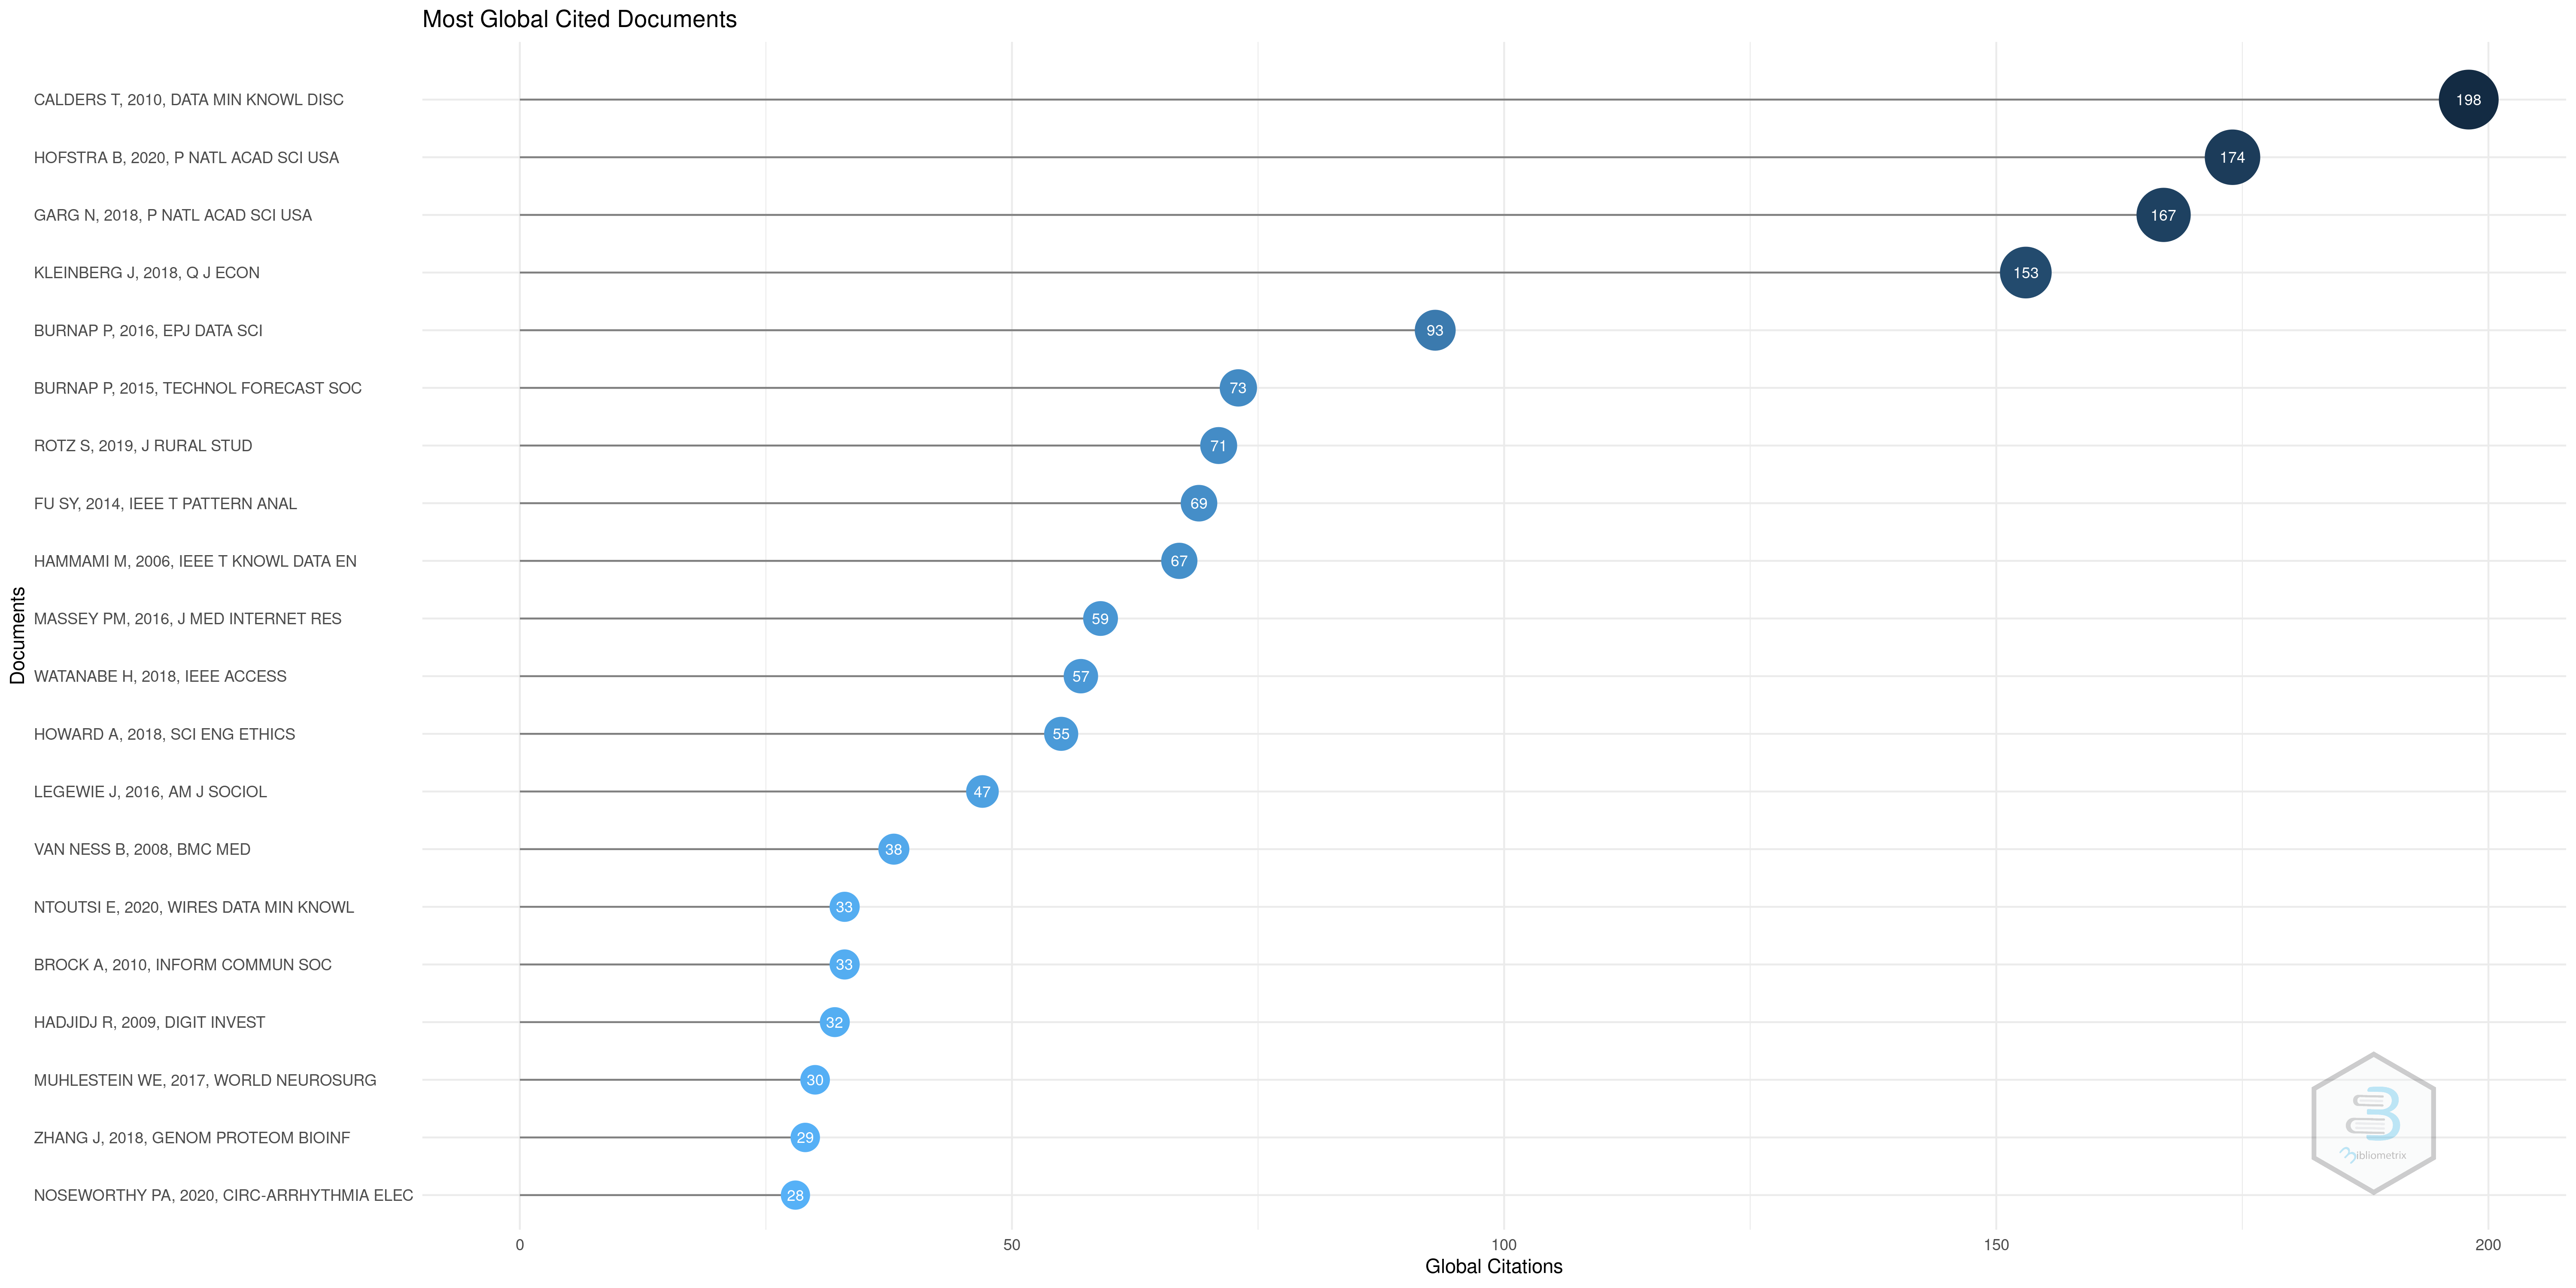
\includegraphics[angle=0,width=1\textwidth]{experiments/gutorsantos/AnaliseBibliometrica/IAeDiscriminacao/imgs/MostGlobalCitedDocuments-2022-02-09.png}
    \caption{Os artigos globais mais citados do IADR@gutorsantos.}
    \label{fig:IADR@gutorsantos:GlobalCitedDocs}
\end{figure}

\begin{figure}[!h]
    \centering
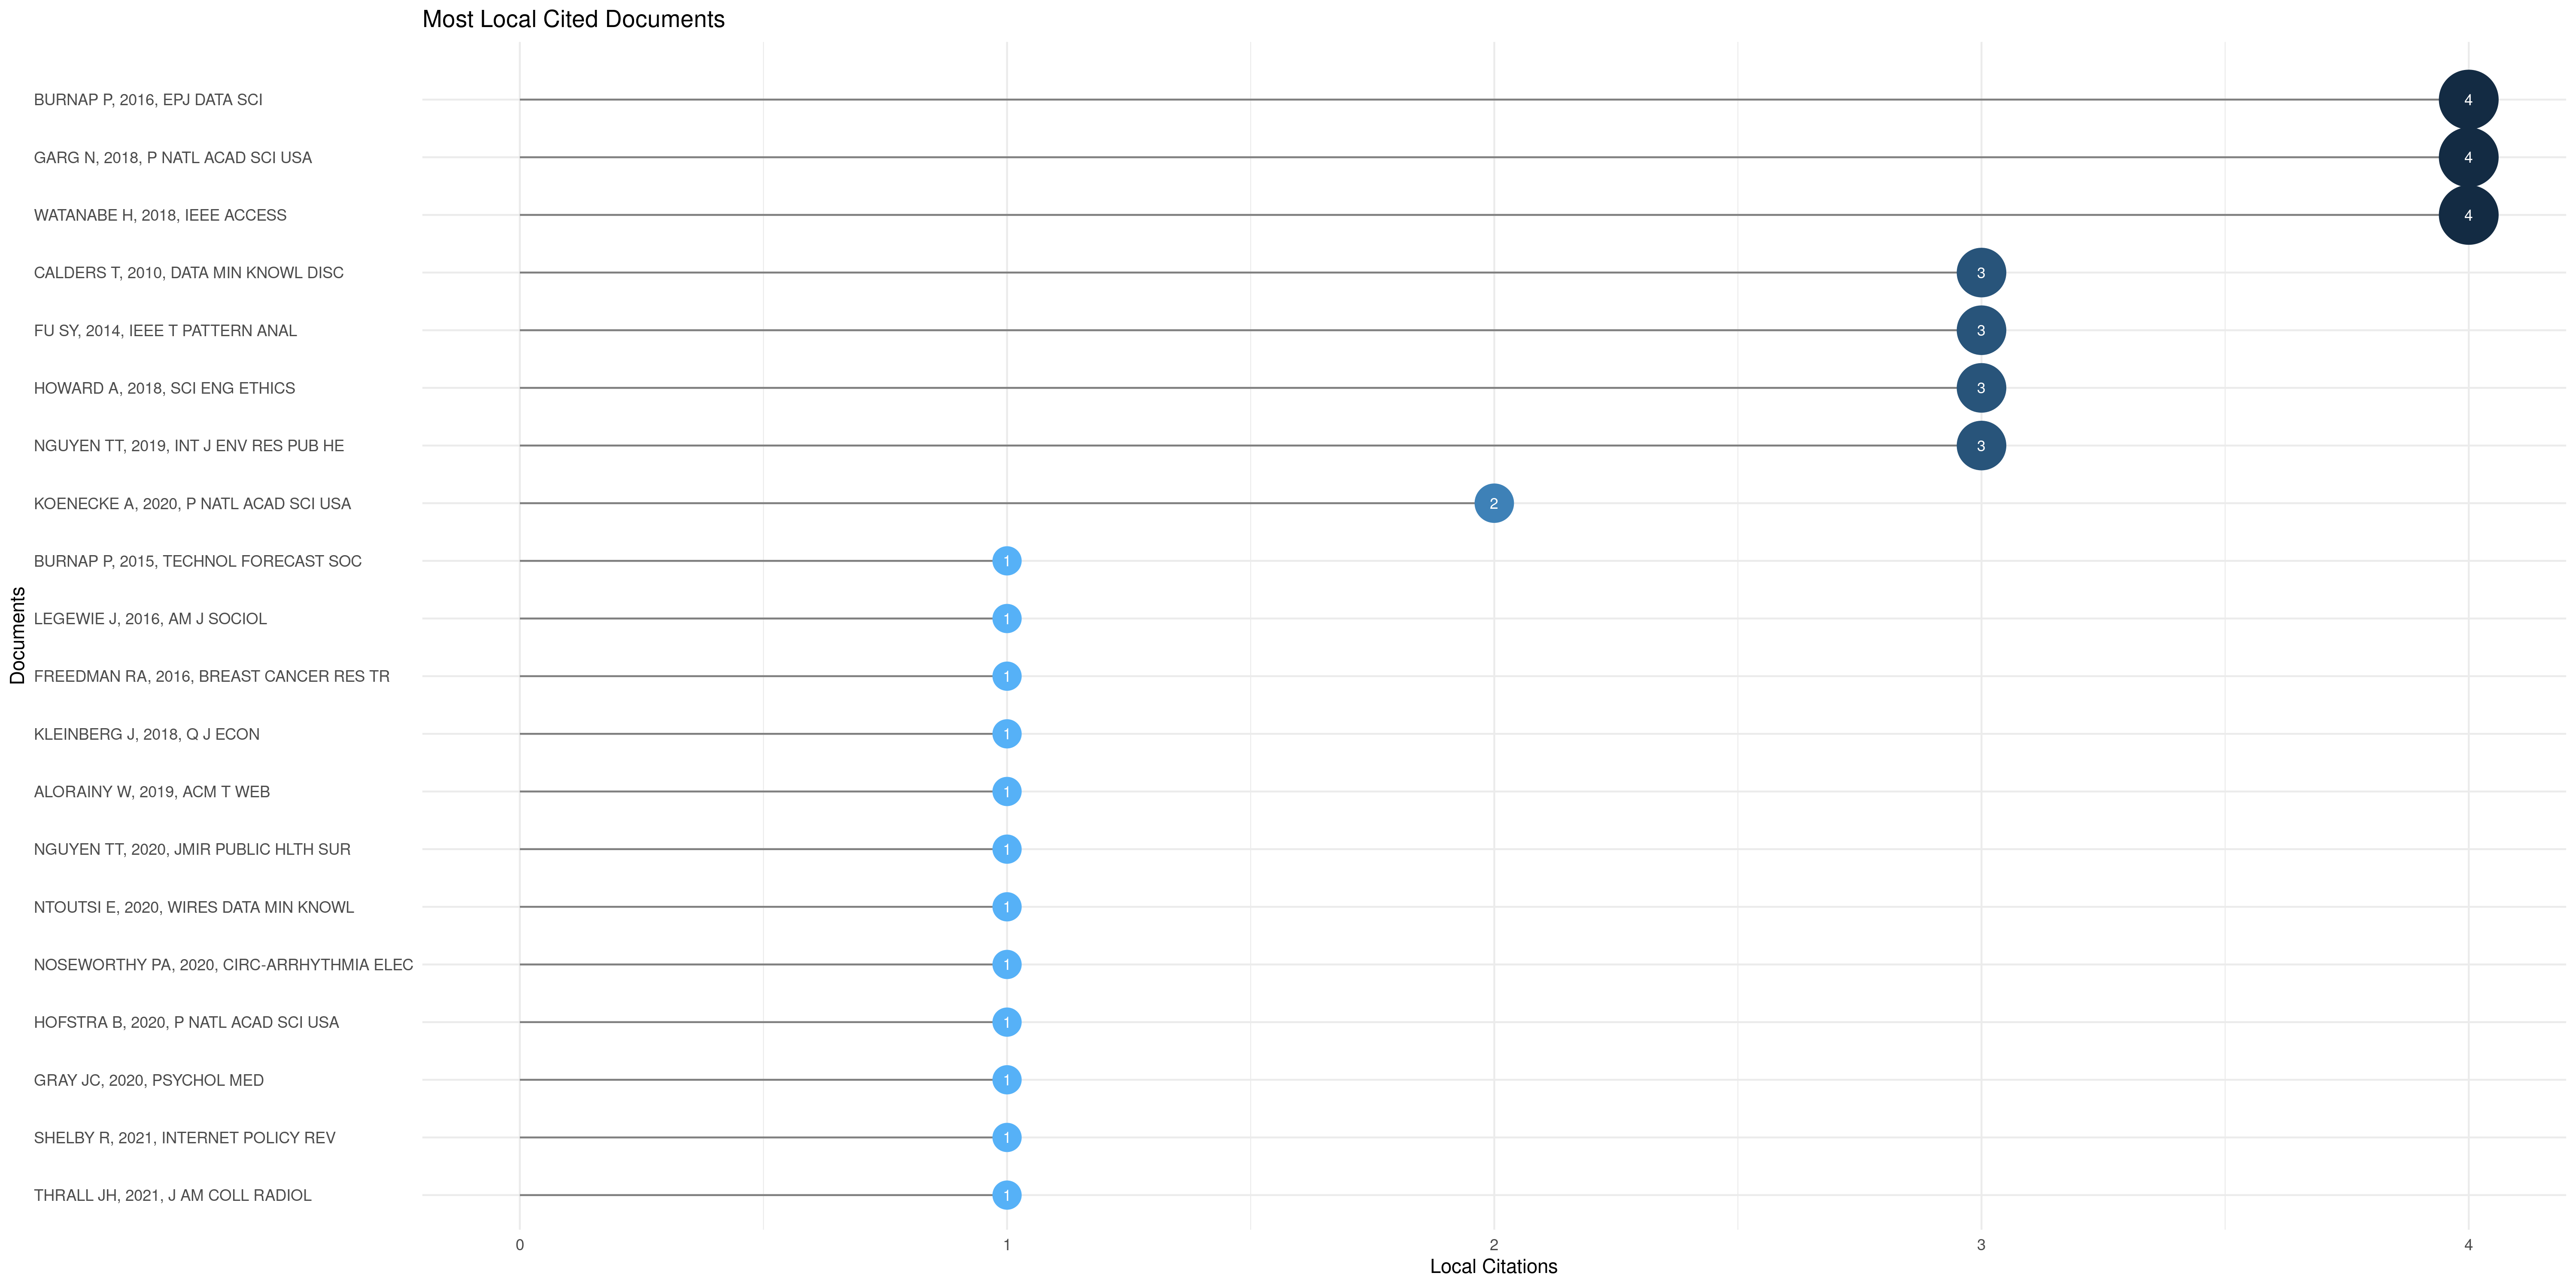
\includegraphics[angle=0,width=1\textwidth]{experiments/gutorsantos/AnaliseBibliometrica/IAeDiscriminacao/imgs/MostLocalCitedDocuments-2022-02-09.png}
    \caption{Os artigos locais mais citados do IADR@gutorsantos.}
    \label{fig:IADR@gutorsantos:LocalCitedDocs}
\end{figure}

Na secção \ref{sec:IADR@gutorsantos:Citations} foi visto que houve um pico de citações em 2010, podemos ver aqui que o artigo em questão é o \textit{``CALDERS T, 2010, DATA MIN KNOWL DISC''}. Ele aparece tanto na figura \ref{fig:IADR@gutorsantos:GlobalCitedDocs} quanto na \ref{fig:IADR@gutorsantos:LocalCitedDocs}, ao encontrá-lo na base de dados, vemos que seu título é \textit{Three naive Bayes approaches for discrimination-free classification} --- Três abordagens de Naive Bayes para classificação livre de discriminação --- portanto, é possível ver que esse artigo é um dos precursores do debate que estamos enfocando, o iniciando no início da década passada, em 2010.

\begin{figure}[!h]
    \centering
    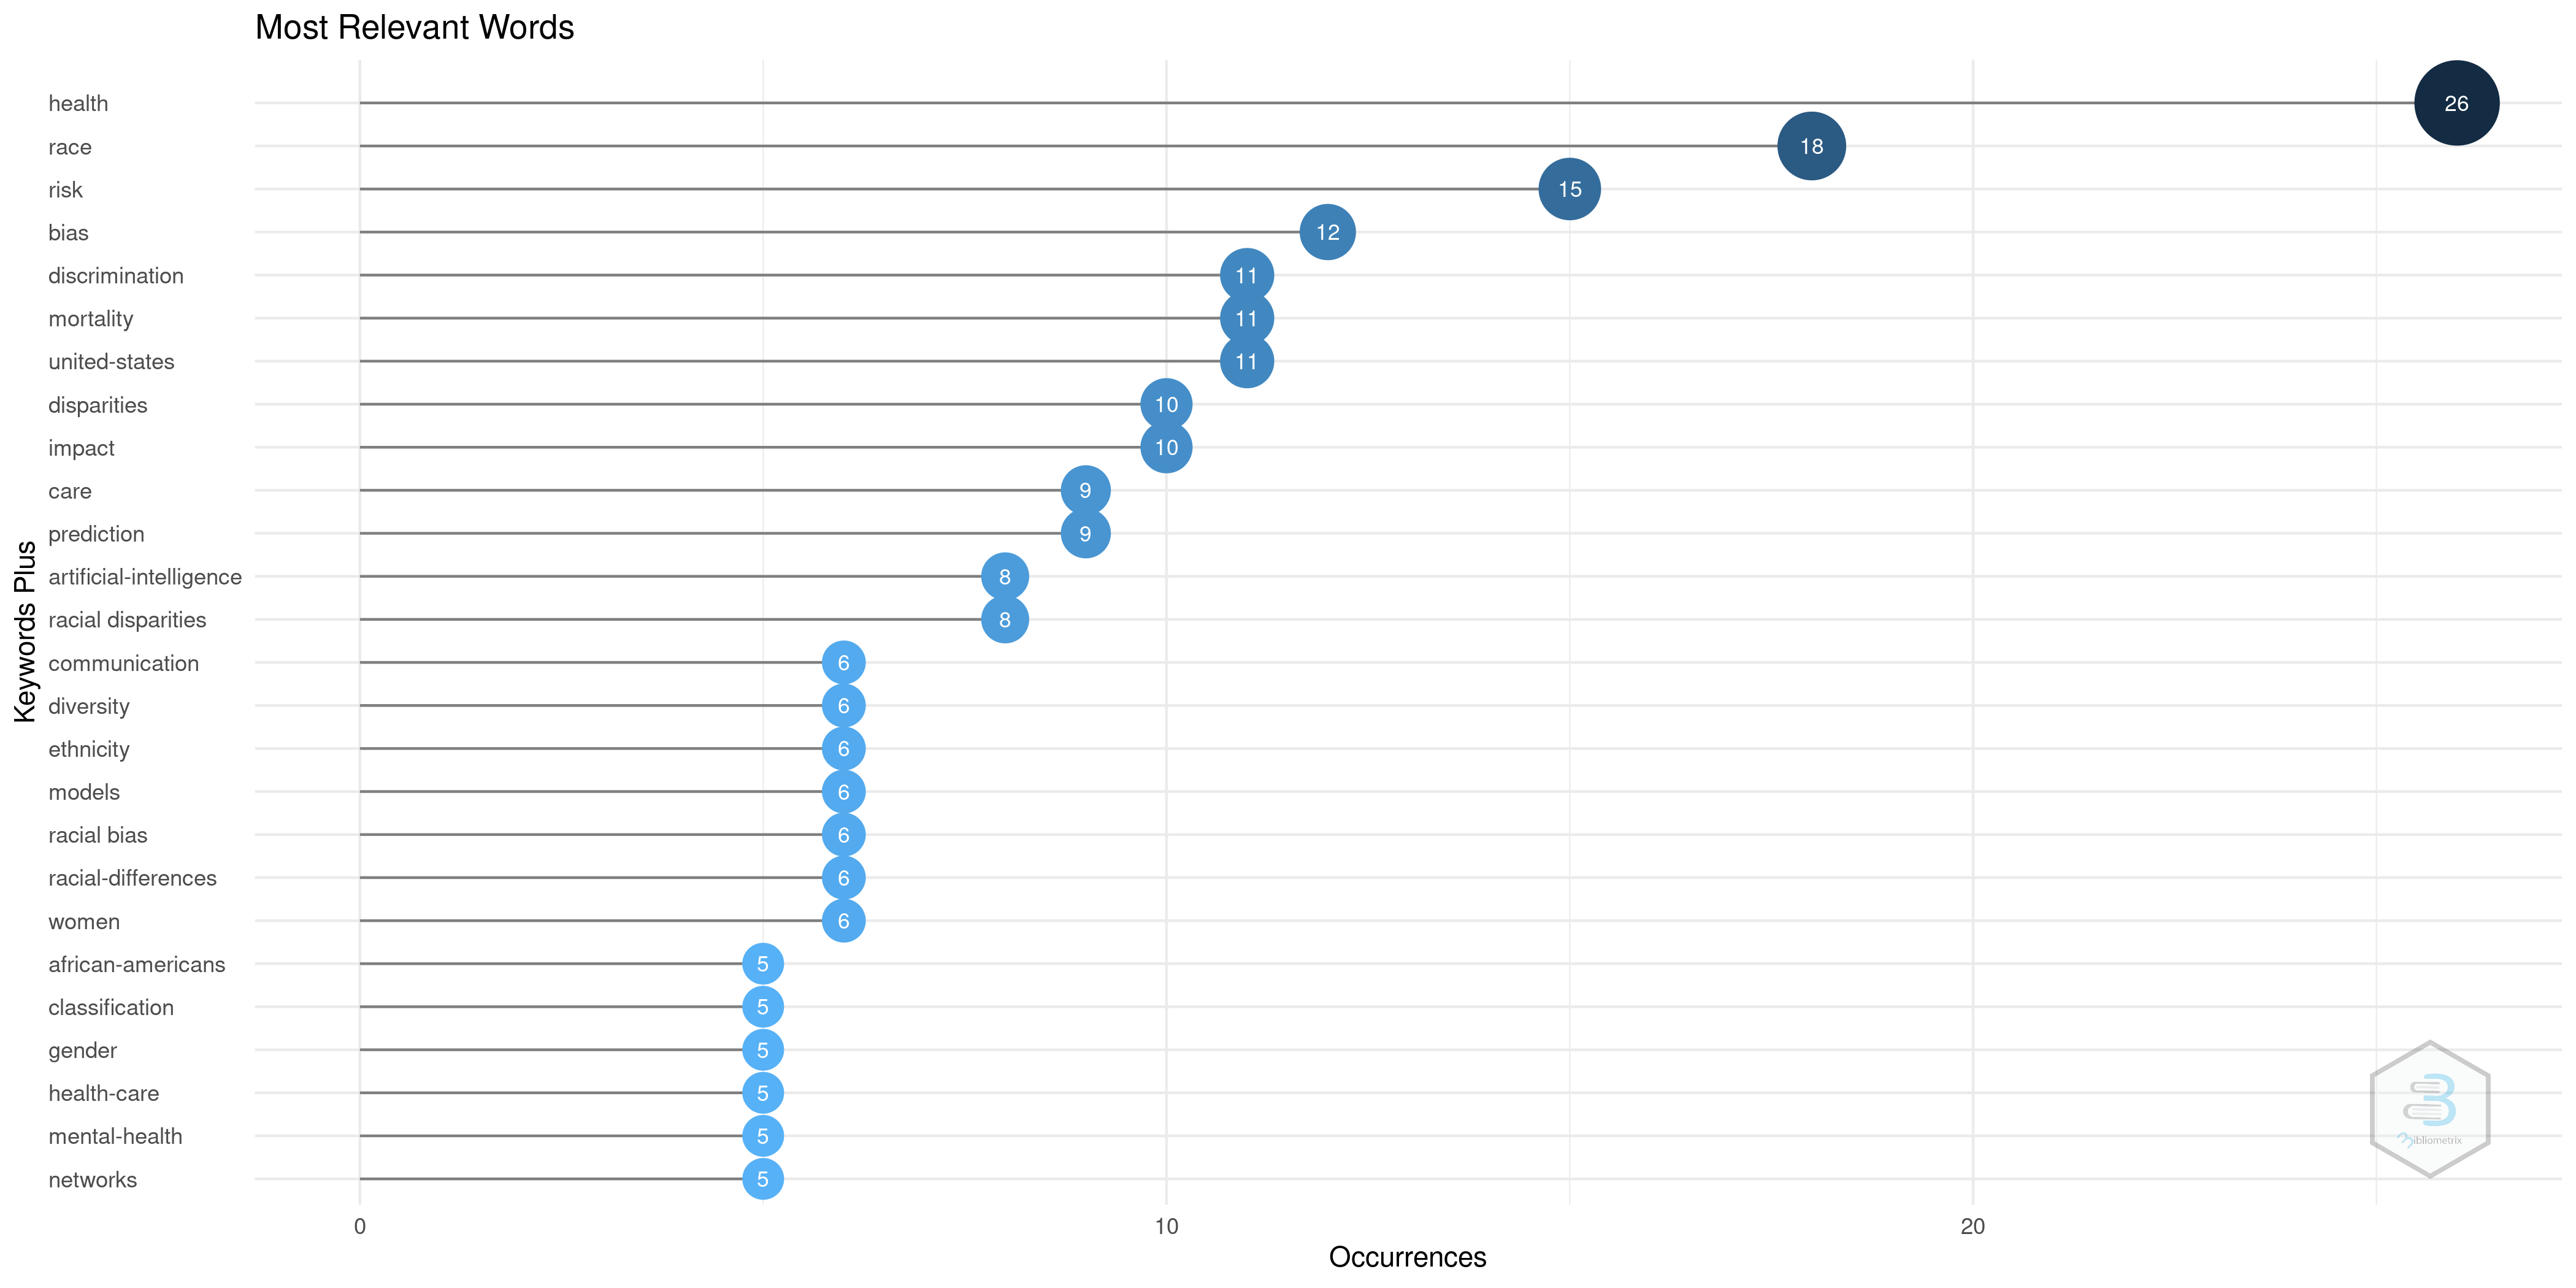
\includegraphics[angle=0,width=1\textwidth]{experiments/gutorsantos/AnaliseBibliometrica/IAeDiscriminacao/imgs/MostRelevantWords-2022-02-09.png}
    \caption{As 20 palavras mais relevantes dentro do dataset IADR@gutorsantos --- utilizando como parâmetro as Keywords Plus}
    \label{fig:IADR@gutorsantos:RelevantWords}
\end{figure}

\begin{figure}[!h]
    \centering
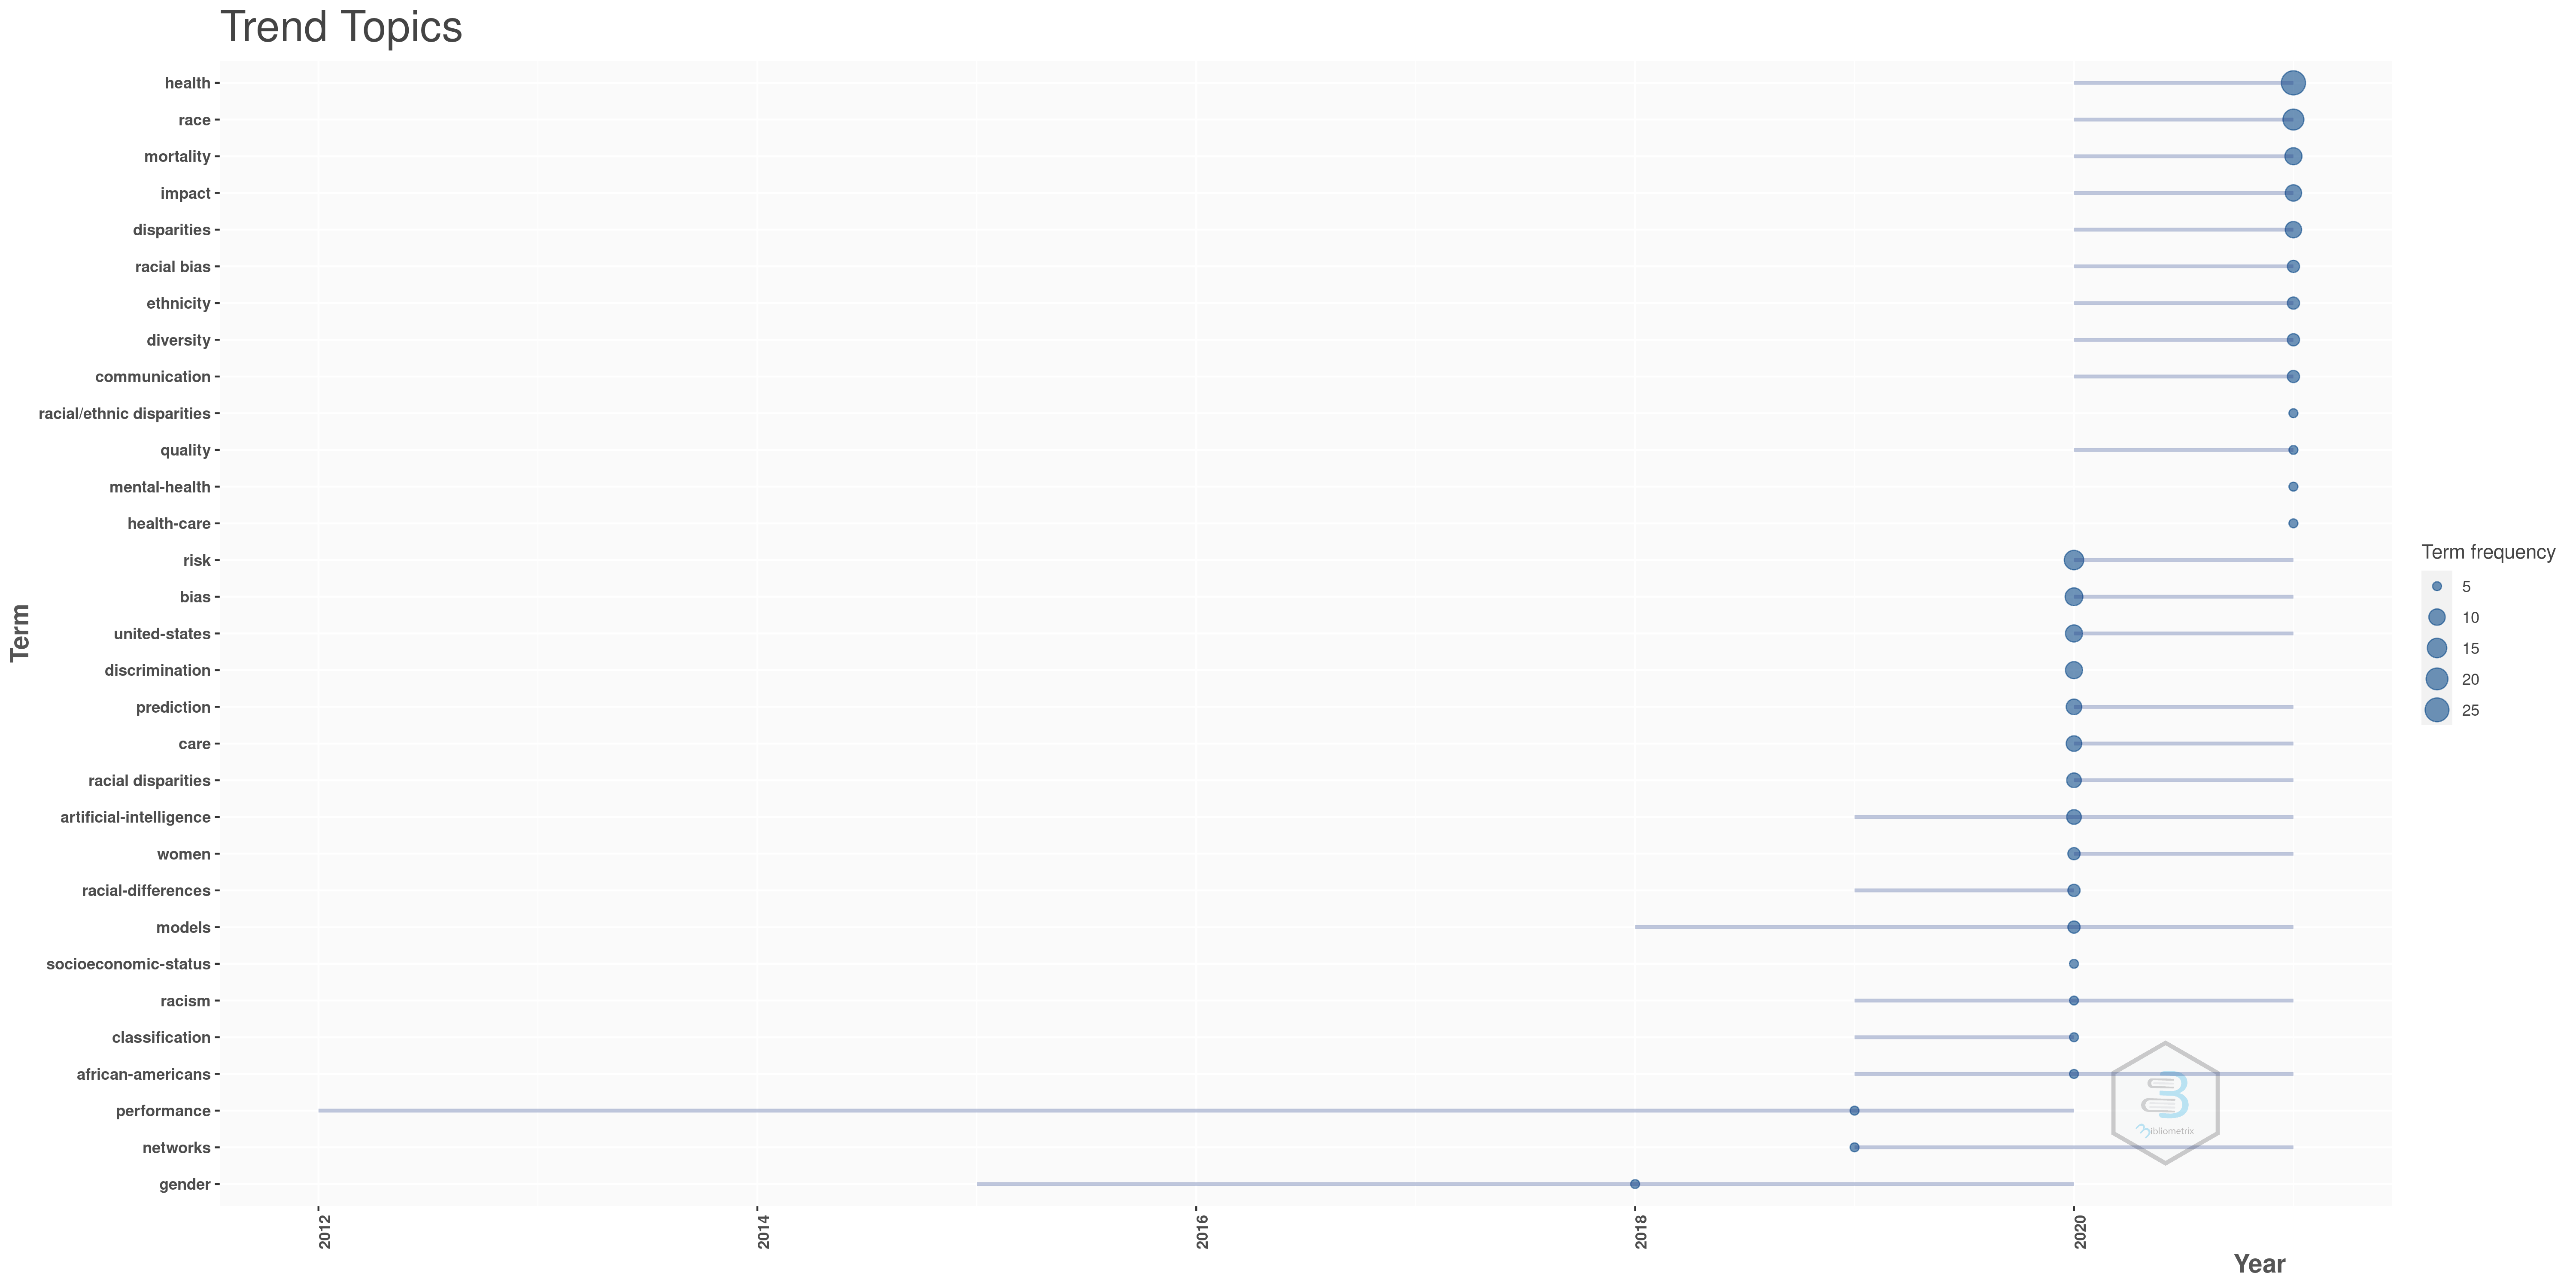
\includegraphics[angle=0,width=1\textwidth]{experiments/gutorsantos/AnaliseBibliometrica/IAeDiscriminacao/imgs/TrendTopics-2022-02-09.png}
    \caption{Tópicos de tendência do dataset IADR@gutorsantos.}
    \label{fig:IADR@gutorsantos:TT}
\end{figure}

A figura \ref{fig:IADR@gutorsantos:RelevantWords} mostra as 20 palavras mais relevantes dentro do contexto do conjunto de dados, extraíndo-as das \textit{Keywords Plus}. Dessa forma, podemos verificar o comportamento já apontado anteriormente, onde é visto o termo \textit{health (saúde)} indicando uma relação dos impactos negativos sobre as populações negras. Note a presença das palavras \textbf{risk (risco)}, \textbf{bias (viés)}, \textbf{discrimination (discriminação)}, \textbf{mortality (mortalidade)} \textbf{disparities (disparidades)}, \textbf{impact (impacto)}, são todas palavras negativas que representam a dimensão perigosa da aplicação da Inteligência Artificial.

Na figura \ref{fig:IADR@gutorsantos:TT}, vemos quando essas palavras se tornam tópicos em destaque, sendo consideradas tendências ou não. Inicialmente, vemos que quase não existem ensaios acadêmicos acerca da questão da discriminação e reforço de preconceitos através de algortimos de IA. Por volta de 2015, surge um ensaio envolvendo questões de gênero. Porém apenas em 2020, são discutidos os problemas do enviesamento dos algoritmos, os riscos e impactos advindos dessa problemática e saúde dos grupos étnicos atingidos. Posto isso, sabe-se que a área de IA vem se desenvolvendo desde o século passado porém é notável que na última década foi quando a Inteligência Artificial teve sua rápida expansão e ascensão. Logo, debates sobre diversidade, igualdade, ética e impactos que deveriam acompanhar a evolução deste artefato tecnológico estão sendo desenvolvidos somente agora, com quase uma década de atraso. 

\subsection{Agrupamento}

